\documentclass[a4paper,12pt]{report}
\usepackage{ngerman}

%neue deutsche Rechtschreibung
%\usepackage[english,ngerman]{babel}

\usepackage[latin1]{inputenc} %f�r Linux
%\usepackage[ansinew]{inputenc} %fuer Windows

\usepackage{mycore}

\begin{document}
%-------   Vorspann
\title{MyCoRe User Guide}
\author{
    Frank L"utzenkirchen\\
    Jens Kupferschmidt\\
    Detlev Degenhardt\\
    Johannes B�hler\\
    Ulrike Kr"onert}
\maketitle
\setcounter{secnumdepth}{10}
\chapter*{Vorwort}
In diesem Dokument sind alle Arbeiten zum Start der Beispielanwendung und zur Gestaltung eigener Anwendungen beschrieben. Teilweise wird auch auf das MyCoRe Design Guide verwiesen.

\pagebreak
\tableofcontents/
\pagebreak
\listoffigures
\pagebreak
\listoftables
\pagebreak
\lstlistoflistings

%-------    Hauptteil
% Kapitel 1
%
%
\chapter{Voraussetzungen f"ur eine MyCoRe Anwendung}
%
%
\section{Vorabbemerkungen}
%
%
Das MyCoRe-Projekt ist so designed, dass es dem Einzelnen Anwender frei steht,
welche Komponenten er f"ur die Speicherung der Daten verwenden will. dabei spielt nat"urlich das verwendete Betriebssystem eine wesentliche Rolle. Dabei hat jeses System eine eigenen Vor- und Nachteile, die an dieser Stelle aber nicht dikutiert werden sollen. Vielmehr wollen wir es dem Anwender "uberlassen, in welchem System er f"ur seine Anwendung die gr"o"sten Vorteile sieht. Nachfolgend finden Sie eine Tabelle der wesentlichen eingesetzten Komponenten entsprechend des gew"ahlten Basissystems. \\[2ex]
\bottomcaption{MyCoRe Komponenten"ubersicht}
\tablehead{\hline}
\tabletail{\hline}
\begin{supertabular}{|p{2cm}|p{3,25cm}|p{3,25cm}|p{3,25cm}|p{3,25cm}|}
\hline
{\bf Teil} & {\bf AIX} & {\bf Solaris} & {\bf Linux} & {\bf MS Windows}\\[1,5ex] \hline
Metadaten Store & IBM CM 8.2 - parametrische und Volltextsuch mittels XPath Abfragen & IBM CM 8.2 - parametrische und Volltextsuch mittels XPath Abfragen & Xindice - parametrische Suche mittels XPath Abfragen & IBM CM 8.2 - parametrische und Volltextsuch mittels XPath Abfragen \\ \hline
TextSearch & IBM DB2 TIE (Sprachunterst�tzung nur f"ur English) & IBM DB2 TIE (Sprachunterst�tzung nur f"ur English) & htdig ??? & IBM DB2 TIE (Sprachunterst�tzung nur f"ur English) \\ \hline
Datenbank & IBM DB2 8.x & Oracle ??? & MySQL 4.x & IBM DB2 8.x \\ \hline
Objekt Store & Filesystem, & Filesystem, & Filesystem, & Filesystem, \\
 & IBM CM 8.2 Ressource Manager, & IBM CM 8.2 Ressource Manager, & & IBM CM 8.2 Ressource Manager, \\ 
 & IBM Video Charger 8, & IBM Video Charger 8, & IBM Video Charger 8, & IBM Video Charger 8, \\
 & Helix Server & Helix Server & Helix Server & Helix Server \\ 
\hline
\end{supertabular}
%
%
\section{Hinweise zur Installation des IBM Content Manager 8.2}
%
%
\subsection{Der IBM Content Manager unter AIX}
An dieser Stelle soll eine Kurzbeschreibung der Installation des IBM Content Managers 8.2 f"ur AIX von Holger K"onig, IBM Deutschland GmbH, wiedergegeben werden. \\[2ex]
\subsubsection{Vorbereitung}
\begin{enumerate}
\item Installieren Sie das AIX Betriebssystem mit dem Release 4.3.3 ML 10, 5.1 ML 01 oder 5.2.
\item Sorgen Sie daf"ur, dass 'Cultural Conversion' und 'Language' auf English US eingestellt ist.
\item Aktivieren Sie die Netzanbindung inklusive DNS.
\item F"ur die Betriebssystem-Releases 4.3.3 und 5.1 muss Java 1.3.1 entsprechend der Anleitung installiert werden. Erweitern Sie in {\it /etc/environment }  die {\it PATH} Variable um {\it /usr/java131/jre/bin} und {\it /usr/java131/bin}.
\item Installieren Sie den VAC Compiler Version 5.x oder 6.0 entsprechend der Anleitung.
\item Aktivieren Sie das Lizenzsystem {\bf ifor} und Tragen Sie sie Compilerlizenzen ein.
\end{enumerate}
\subsubsection{DB2 und NSE}
\begin{enumerate}
\item Kopieren Sie das File {\it ese.sbcs.tar.Z} von der CD {\bf 'DB2 8.1 with FP1'} und entpacken Sie dieses.
\item {\tt ./db2setup}
\item W"ahlen Sie {\bf Install Products} $\rightarrow$ {\bf DB2 UDB Enterprise Server Edition}. Folgen Sie den Schritten:
\begin{itemize}
\item {\bf Netx}
\item {\bf Accept License}
\item Select 'Custom' $\rightarrow$ {\bf Next}
\item Select 'Install DB2 UDB Enterprise Server Edition on this computer' $\rightarrow$ {\bf Next}
\item Select 'Appliction Development Tools' zus"atzlich
\item Sprache 'Englisch' beibehalten $\rightarrow$ {\bf Next}
\item Erzeugen der DB2 Instanz durch Select 'Create a DB2 instance - 32 bit' $\rightarrow$ {\bf Next}
\item Select 'Single-partition instance' $\rightarrow$ {\bf Next}
\end{itemize}
\end{enumerate}
%

%
%
\subsection{Der IBM Content Manager unter Solaris}

%
%
\subsection{Der IBM Content Manager unter Windows}

%
%
\section{Hinweise zur Installation frier Datenbanken und XML:DB's}

%
%
\subsection{Die Installation von MySQL}

%
%
\subsection{Die Installation von Xindice}

%
%
\section{Hinweise zur Arbeit mit der Servlet-Engine}

%
%
\subsection{Arbeiten mit Tomcat}

%
%
\subsection{Arbeiten mit Websphere}

%
%
\section{Weitere erforderliche Software}



% Kapitel 2
%
%
\chapter{Download und Installation des MyCoRe Kerns}
%
%
\section{Download des MyCoRe Kerns}
%
%
Das MyCoRe Projekt wird f"ur alle unterst"utzten Systeme "uber das CVS Repository
ausgeliefert. Das Holen der aktuellen Version erfolgt mit dem Kommando 
\begin{center}
{\tt cvs -d :pserver:anoncvs@server.mycore.de:/cvs checkout mycore} 
\end{center}
Nach dem erfolgreichen Checkout erhalten Sie folgende Dateistruktur:\\[2ex]
\bottomcaption{Dateistruktur des MyCoRe Kernes}
\tablehead{\hline}
\tabletail{\hline}
\begin{supertabular}{|p{5cm}|p{10cm}|}
\hline
{\bf mycore} &  Das Root-Verzeichnis des MyCoRe-Kerns \\
\quad {\bf bin} & Das Verzeichnis der Shellscripte \\
\qquad build.sh & Shellscript zum Compilieren unter einem UNIX-System \\
\qquad build.cmd & Shellscript zum Compilieren unter einem UNIX-System \\
\qquad mycore.sh & Shellscript zur Arbeit mit dem Commandline-Interface unter UNIX \\
\qquad mycore.cmd & Shellscript zur Arbeit mit dem Commandline-Interface unter Windows \\
\qquad setup\_cm7.sh & Shellscript f"ur eine UNIX-Umgebung mit IBM Content Manager 7 \\
\qquad setup\_cm7.cmd & Kommandoscript f"ur eine Windows-Umgebung mit IBM Content Manager 7 \\
\qquad setup\_cm8.sh & Shellscript f"ur eine UNIX-Umgebung mit IBM Content Manager 8.1/8.2 \\
\qquad setup\_cm8.cmd & Kommandoscript f"ur eine Windows-Umgebung mit IBM Content Manager 8.1/8.2 \\
\qquad setup\_xindice.sh & Shellscript f"ur eine UNIX-Umgebung mit Xindice \\
\qquad setup\_xindice.cmd & Kommandoscript f"ur eine Windows-Umgebung mit Xindice \\
\quad {\bf documentation} & Dokumentationen zu MyCoRe \\
\quad {\bf lib} & Noterndige zus"atzliche Java-Bibliotheken \\
\quad {\bf schema} & XMLSchema Dateien, die anwendungsunabh"angig sind \\
\quad {\bf sources/org/mycore} & Die Wurzel des MyCoRe-Source-Baumes \\
\qquad {\bf datamodel} & Klassen zum Datenmodell \\
\quad \qquad {\bf classifications} & Klassen zur Arbeit mit den Klassifikationen \\
\quad \qquad {\bf ifs} & Klassen zur Arbeit mit dem Internal File System \\
\quad \qquad {\bf metadata} & Klassen zur Arbeit mit den Metdaten \\
\qquad {\bf common} & Klassen, die im gesamten Projekt ben�tigt werden \\
\quad \qquad {\bf xml} & Allgemeine Klassen zur XML Verarbeitung \\
\qquad {\bf backend} & Klassen f"ur die verschiedenen Data Stores \\
\quad \qquad {\bf cm7} & Klassen zur Nutzung des IBM Content Manager 7 \footnote{Die Klassen f�r den IBM Content Manager 7 werden nicht merh weiterentwickelt!} \\
\quad \qquad {\bf cm8} & Klassen zur Nutzung des IBM Content Manager 8.2 \\
\quad \qquad {\bf filesystem} & Klassen zum Content Store im lokalen Filesystem \\
\quad \qquad {\bf realhelix} & Klassen zum Content Store in einem Helix-Server \\
\quad \qquad {\bf remote} & Klassen zum Zugriff auf Remote-MyCoRe-Daten \\
\quad \qquad {\bf sql} & Klassen zum Zugriff auf relationale Datenbanken mittels SQL-Standart \\
\quad \qquad {\bf videocharger} & Klassen zum Content Store in einen IBM Videocharger \\
\qquad {\bf frontend} & Klassen f"ur die Frontends des MyCoRe-Systems \\
\quad \qquad {\bf cli} & Klassen des Commandline-Tools \\
\quad \qquad {\bf editor} & Klassen zug Gestaltung von Editoren \\
\quad \qquad {\bf servlets} & Klassen zu Gestaltung von Servlets \\
\qquad {\bf services} & Klassen f"ur weiterf"uhrende Services des MyCoRe-Projektes \\
\quad \qquad {\bf nbn} & Klassen zur Arbeit mit NBN's \\
\quad \qquad {\bf oai} & Klassen zur Arbeit mit OAI Komponenten \\
\quad \qquad {\bf query} & Klassen zur Arbeit mit dem MyCoRe internen Query-System \\
\qquad {\bf user} & Klassen des User- und Rechteverwaltungssystems \\
\quad build.xml & Konfigurations-File f�r die Arbeit mit ANT \\
\quad license.txt & Das Lizenz-File des MyCoRe-Projektes, bitte lesen Sie dieses File aufmerksam durch, bevor Sie MyCore einsetzen. \\
\hline
\end{supertabular}
%
%
\section{Konfiguration und "Ubersetzten des Kerns}
%
%
Nach dem checkout der Files muss als erstes dieses Paket "ubersetzt werden. Die Arbeit erfolgt in den unten angegebenen Schritten.\\
\begin{enumerate} 
\item Zur Anpassung der erforderlichen Umgebung gibt es zwei Wege. Entweder alle notwendigen Variablen wie CLASSPATH usw. werden in den entsprechenden Nutzer-Profile gesetzt oder ({\bf empfohlen}) sie setzen an dieser Stelle nur die Environment-Variable {\bf MYCORE\_HOME} in Ihrer Systemumgebung und kopieren das entsprechende Template {\it setup\_....sh} (bzw. {\it setup\_....cmd}) im Verzeichnis {\it bin} dort nach {\it setup.sh} (bzw. {\it setup.cmd} f"ur die Windows Plattform) F"ur die unterst"utzten Systeme stehen jeweils entsprechende Files bereit. Passen Sie nun das Setup-Script an die eigene Konfiguration hinsichtlich der ben"otigten Software (Pfade zu ANT, Java usw.) an. 
\item Als n"achstes ist im File {\it \$MYCORE\_HOME/build.xml} die Zeile \\
\begin{center}
{\tt <property name=\grq\grq persistency\grq\grq  value=\grq\grq cm7\grq\grq />} 
\end{center}
entsprechend des gew"ahlten Persistence-Layers anzupassen. M"ogliche Werte sind {\it cm7}, {\it cm8} und {\it xmldb}.
\item Starten Sie nun die "Ubersetzung mit einem Aufruf von {\it ant} oder ({\bf empfohlen}) der Ausf"uhrung des Shell-Scripts {\it bin/build.sh} (bzw. {\it bin/build.cmd}). Bei der Abarbeitung des Kommandos ohne Parameter wird Ihnen eine Auswahl an m"oglichen Parametern angeboten. So k"onnen Sie hier zum Beispiel alle Klassen kompilieren oder nur die Javadoc-Dokumentation bzw. diese Dokumentation erstellen. 
\item Um die f"ur die MyCoRe-Anwendung ben"otigten Java-Klassen zu erzeugen starten Sie einfach \\
\begin{center}
{\it \$MYCORE\_HOME/bin/build.sh jar }
\end{center} 
\end{enumerate} 
Abh"angig von Ihrer Wahl beim build werden weitere Unterverzeichnisse im Verzeichnisbaum unter {\it \$MYCORE\_HOME} erstellt: 
\begin{itemize} 
\item mycore/classes $\longrightarrow$ enth"alt die Java Klassen 
\item mycore/javsadocs $\longrightarrow$  enth"alt die Java Dokumentation 
\end{itemize} 
%
%

% Kapitel 3
\chapter{Die MyCore Beispielanwendung}
% Abschnitt 3.1
%
%
\section{Grundlegender Aufbau und Ziel der Beispielanwendung}
%
%
\subsection{Allgemeines}
Um die Funktionsweise des MyCoRe-Kernes zu testen wurde eine Beispielanwendung basiered auf diesem Kern entwickelt. Sie soll dem Anwender eine voll funktionsf"ahige Applikation in die Hand geben, welche eine Vielzahl von Komponenten des MyCoRe-Projektes nutzt und deren Arbeitweise klar werden l"asst. Um die Anwendung, im weiteren MyCore-Sample genannt, gleichzeitig sinnvoll einsetzten zu k"onnen, wurde als Beispielszenario ein Dokumentserver gew"ahlt, wie er bei vielen potentiellen Nutzern zur Anwendung kommt. Auch soll das MyCore-Sample die Nachfolge des erfolgreichen MILESS-Dokumentservers sein und den Migrationspfad zu MyCoRe hin aufzeigen. \\[2ex]
Analog zum MILESS werden auch hier die Metadaten in drei Gruppen aufgeteilt und von den eigentlichen multimedialen Objekten getrennt behandelt. Zur Modellierung des Datenmodells f"ur die Multimedia-metadaten wurde das allgemein verbreitete Dublin Core Datenmodell herangezogen und umgesetzt. Zur Realisierung wurden folgende Metadaten-Objekte entwickelt:
\begin{itemize}
\item {\bf Document} - Dieses Objekt beinhaltet die eigentlichen Metadaten des Multimedi-Objektes, in unserem Fall im Dublin Core Format, sowie Verweise auf extern gehaltene Daten wie die drei im weiteren genannten. Das Datenmodell besteht aus 15 Feldern, zur Speicherung verschiedener Datentypen gibt es atomare Grundkomponenetn. Weiterhin beinhalten die Metaddaten noch Teile zu ihrer Struktur und Verwaltung.
\item {\bf Klassifikation} - Hier k"onnen lineare oder hierarchich strukturierte Klassifikationen mit ihren Kategorien abgelegt werden. Jeder Verweis auf eine solche Kategorie aus einem Dokument heraus erfolgt mittels der ID der selben und nat"urlich der ID der Klassifikation als Identifiziererpaar. F"ur die Gestaltung der Klassifikationen wurde ein eigens Datenmmodel entwicklet.
\item {\bf LegalEntity} - Auch diese Metadaten sind analog dem {\bf Document} aus atomaren Komponenten zusammengesetzt und repr"asentieren nat"urliche und juristische personen, wie Autoren oder Einrichtunge.
\item {\bf Derivate} - Hinter diesem Begriff verbergen sich Darstellungsformen der eigentlichen multimedialen Objekte. Beispielsweise k"onnen das verschieden Dateiformate eines Images sein. Diese werden an das eigentliche Dokument gebunden.
\end{itemize}
Eine "Ubersicht zu den Beziehungen der Objektteile zueinander soll die folgende Grafik vermitteln. Wir haben uns aus den guten Erfahrungen von MILESS herraus entschlossen, diese Aufteilung beizubehalten, da so Einzelkomponeneten in Projekten schon geladen werden k"onnen, bevor andere Teile, z. B. das Scannen, abgeschlossen sind. \\
\begin{figure}[H]
\begin{center}
\fbox{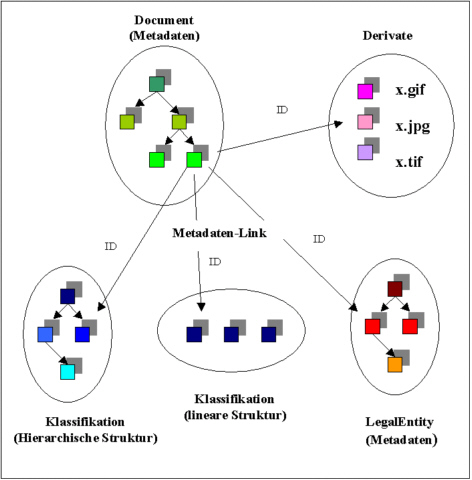
\includegraphics[scale=0.8]{UserGuide_3Goals_Pic01.jpg}}
\caption{"Ubersicht der Objekte im MyCoRe-Sample}
\end{center}
\end{figure}
Wie man der Grafik entnehmen kann, ist es m"oglich, neben Kategorien in Klassifikationen auch Metadaten der Documnets und LegalEntities hierarchich ineienander zu verschachteln. Auf dieser Basis k"onnen dann Strukturen wie z. B. die eines Buches abgebildet werden. Alle Beziehungen zwischen den Metadaten sind "uber eine eindeutige MCRObjectID gel"ost. \\
\subsection{Die MCRObjectID}
Dreh- und Angelpunkt aller Beziehungen von Metadaten und der daran angekn�pften Objekte ist ein eindeutiger Identifizierer. Im Falle des MyCoRe Projektes hat dieser den Namen {\bf MCRObjectID} erhalten. Er hat f�r alle Matadaten einen einheitlichen Aufbau und wird st�ndig zur Identifizierung genutzt. Auch das API des Systems bietet die M�glichkeit, diese ID automatisch zu generieren.\footnote{Siehe Programmers Guide.} Der Syntax der {\bf MCRObjectID} ist wie folgend festgelegt:\\
\begin{center}
{\bf MCRObjectID = {\it project\_type\_number}}
\end{center}
{\it project} - Dieses Element der ID spezifiziert ein bestimmtes Projekt. Es dient dazu, Daten verschiedener Projekte, welche sich gemeinsam auf einem System befinden, zu unterscheiden. Der Projektname sollte eindeutig sein und besteht aus einem Wort {\bf ohne Sonderzeichen}. Achten Sie immer darauf, dass Sie sich bei Vorhaben mit mehreren MyCoRe-Partnern von Anfang an auf einen Namen pro Projektteilnehmer verst�ndigen. F�r unser Sample haben wir {\bf MyCoReDemoDC} ausgew�hlt. {\bf Dieser Teil der ID ist case sensitive!}\\[2ex]
{\it type} - Jedem Metadatentyp des Datenmodells ist ein Typbezeichner zuzuordnen. Dieser stellt in MyCoRe die Verbindung von der Konfiguration des Metadatums bis hin zu dessen Suche und Pr�sentation dar. Der Typname der MCRObjectID wird immer in Kleinbuchstaben (lower case) innerhalb des Systems verwendet. Achten Sie von Anfang an darauf, dies umzusetzen. Im MyCoRe-Projekt gibt es reservierte Typnamen, diese sind\\
\begin{itemize}
\item {\bf class} - f�r Klassifikationen
\item {\bf derivate} - f�r Derivate
\end{itemize}
Zur Umsetztung des Datenmodells wurden weiterhin die Typen {\bf document} f�r Dokumente und {\bf legalentity} f�r Personen verwendet.
{\it number} - Dieser Teil dient der Identifizierung des Einzelobjektes. Es d�rfen nur nat�rliche Zahlen angegeben werden. Planen Sie Ihre Vergabe der Nummern bei eigenen Objekten sorgf�ltig. Da die Nummern teilweise als Strings verarbeitet werden, ist es sinnvoll, sie mit einer ausreichenden Zahl von Vornullen zu versehen. Dies erledigt das MyCoRe-System automatisch unter Zuhilfenahme des Konfogurationswertes {\tt MCR.metadata\_objectid\_number\_pattern } im File {\it mycore.properties.private }.
\subsection{Das Sample-Datenmodell}
Das Datenmodell des MyCoRe-Samples soll exemplarisch einen kleinen Dokumentserver abbliden, wie er dann f�r gro�e L�sungen �bernommen werden kann. Dabei sollen Multimediale Objekte verschiedenster Art und Herkunft gemeinsam verwaltet werden. Als Grundger�st f�r die Dokumente diente uns das Dublin Core Datenmodell, welches in einigen Punkten inhaltlich etwas nach unseren Auffassungen angepasst wurde. Das Personen-Datenmodell ist hingegen derzeit propit�r. Ggf. kommen hier in einer sp�teren version von MyCoRe Standard-Datenmodelle zum Einsatz. Die Klassifikationen sind hierarchich angelegt, d. h. Kategorien k�nnen wieder Unterkategorien beherbergen. Im folgenden werden die einzelnen Felder des Metadatenmodelles beschrieben und es wird aufgezeigt, welche Suchen vorgesehen sind. Dabei bedeutet PS - parametrische Suche, TS - Volltextsuche. Eine genaue Beschreibung der Suchmechanismen finden Sie im Programmers Guide. \\[2ex]
{\bf Die Klassifikationen (Classifications)}  \\[2ex]
F�r das Datenmodell sind die folgenden Klassifikationen vorgesehen. Alle Label und Descriptions der einzelnen Kategorien k�nnen dabei in mehreren Sprachen angegeben werden.
\begin{itemize}
\item {\bf Format} - enth�lt eine einfache Liste der m�glichen Formate des Dokumentes.
\item {\bf Typen}  - enth�lt eine einfache Liste der m�glichen Typen des Dokumente.
\item {\bf Einger} - enth�lt eine hierarchiche Liste aller m�glichen Eignergruppen eines Dokumentes.
\end{itemize}


{\bf Das Dokument (Document)}  \\[2ex]
\small
\bottomcaption{Das Document Datenmodell}
\tablehead{\hline}
\tabletail{\hline}
\begin{center}
\begin{supertabular}{|p{2cm}|p{4cm}|p{9cm}|}
\hline
{\bf Bezeichner} & {\bf Type} & {\bf Beschreibung} \\[1,5ex] \hline
Title & MCRMetaLangText & Titel des Werkes, alternative Titel usw. in mehreren Sprachen\\ \hline
Creator & MCRMetaLink & Enth�lt eine Liste von Links auf Autoren, Erzeuger, Einrichtungen usw. \\[1,5ex] \hline
Subject & MCRMetaClass & Subjekte, die in Form von Klassifikationen vorliegen. Dies k�nnen z. B. Schlagworte sein. \\ \hline
Description & MCRMetaLangText &  Eine verbale Kurzbeschreibung des Objektes, ggf. ist diese in verschiedenen Sprachen gehalten.\\ \hline
Publisher & MCRMetaLink & Enth�lt eine Liste von Links auf Personen und deren Institutionen, die an der Ver�ffentlichung des Objektes beteiligt waren.\\ \hline
Contributor & MCRMetaLink & Enth�lt eine Liste von Links auf Personen und deren Institutionen, die anderweitig am Entstehen des Objektes beteiligt waren.\\ \hline
Date & MCRMetaDate & Datumsangaben zum Objekt. \\ \hline
Type & MCRMetaClass & Type des Objktes. \\ \hline
Format & MCRMetaClass & Angaben �ber die physikalischen Eigenschaften des physischen Objektes.\\ \hline
Identifier & MCRMetaLangText & Inventarnummern und Angaben zur physikalischen Aufbewahrung des Objektes.\\ \hline
Source & MCRMetaLangText & Quellen und Erwerbsangaben des physikalischen Objektes, ggf. in mehreren Sprachen.\\ \hline
Language & Entf�llt, wird innerhalb der einzelnen Metadaten abgelegt. & Angaben �ber die Sprache, in der das physikalische Objekt gehalten ist. \\ \hline
Keywords & MCRMetaLangText & Schl�sselworte f�r die Suche, ggf. in mehreren Sprachen. \\ \hline
Coverage & MCRMetaLangText & Zeitliche und r�umliche Erstreckung des Werkes, ggf. in mehreren Sprachen. \\ \hline
Rights & MCRMetaLangText & Text zu den Rechten eines Werkes, ggf. in mehreren Sprachen.\\ \hline
\end{supertabular}

\end{center}\normalsize

\small
\bottomcaption{Das Document Suchmodell}
\tablehead{\hline}
\tabletail{\hline}
\begin{center}
\begin{supertabular}{|p{8cm}|p{2cm}|p{2cm}|}
\hline
{\bf relativer Pfad} & {\bf PS} & {\bf TS}\\[1,5ex] \hline
ID & $\surd$ & - \\ \hline
label & $\surd$ & - \\ \hline
structure/derobjects/derobject & $\surd$ & - \\ \hline
structure/parents/parent  & - & - \\ \hline
structure/children/child  & - & - \\ \hline
metadata/titles/title & $\surd$ & $\surd$ \\ \hline
metadata/creators/creator & $\surd$ & - \\ \hline
metadata/subjects/subject & $\surd$ & - \\ \hline
metadata/descriptions/description & $\surd$ & $\surd$ \\ \hline
metadata/publishers/publisher & $\surd$ & - \\ \hline
metadata/contributors/contributor  & $\surd$ & - \\ \hline
metadata/dates/date & $\surd$ & - \\ \hline
metadata/types/type & $\surd$ & - \\ \hline
metadata/formats/format & $\surd$ & - \\ \hline
metadata/identifiers/idenifier & $\surd$ & - \\ \hline
metadata/sources/source & - & - \\ \hline
metadata/keywords/keyword  & $\surd$ & $\surd$ \\ \hline
metadata/coverages/coverage  & $\surd$ & $\surd$ \\ \hline
metadata/rights/right & $\surd$ & - \\ \hline
service/servdates/servdate & $\surd$ & - \\ \hline
service/servflags/servflag & $\surd$ & - \\ \hline
\end{supertabular}

\end{center}\normalsize

{\bf Die Personendaten (LegalEntities)}  \\[2ex]
\small
\bottomcaption{Das Personen Datenmodell}
\tablehead{\hline}
\tabletail{\hline}
\begin{center}
\begin{supertabular}{|p{2cm}|p{4cm}|p{9cm}|}
\hline
{\bf Bezeichner} & {\bf Type} & {\bf Beschreibung} \\[1,5ex] \hline
Person & MCRMetaPerson & Name einer Person mit akademischen Titel, Adelstitel, Namen, Vornamen und ggf. Typ des Namens (Alias usw.).\\ \hline
Corporation & MCRMetaCorporation & Name einer Institution oder Einrichtung mit Bereichs- und Abteilungsbezeichnungen und ggf. Typ des namens. \\ \hline
Address & MCRMetaAddress & Die Adresse mit Land, Staat, Ort, PLZ, Stra�e und Nummer.\\ \hline
Date & MCRMetaDate & Datumsangaben.\\ \hline
Phone & MCRMetaLangText & Die Telefonnummern.\\ \hline
WEB & MCRMetaLangText & Die Web Adressen.\\ \hline
eMail & MCRMetaLangText & Die eMail Adressen.\\ \hline
\end{supertabular}
\end{center}
\normalsize

\begin{center}
\small
\bottomcaption{Das LegalEntity Suchmodell}
\tablehead{\hline}
\tabletail{\hline}
\begin{supertabular}{|p{8cm}|p{2cm}|p{2cm}|}
\hline
{\bf relativer Pfad} & {\bf PS} & {\bf TS}\\[1,5ex] \hline
ID & $\surd$ & - \\ \hline
label & $\surd$ & - \\ \hline
structure/derobjects/derobject & $\surd$ & - \\ \hline
structure/parents/parent  & - & - \\ \hline
structure/children/child  & - & - \\ \hline
metadata/persons/person & $\surd$ & $\surd$ \\ \hline
metadata/corporations/corporation & $\surd$ & $\surd$ \\ \hline
metadata/addresses/address & $\surd$ & - \\ \hline
metadata/dates/date & $\surd$ & - \\ \hline
metadata/phones/phone & - & - \\ \hline
metadata/webs/web & - & - \\ \hline
service/servdates/servdate & $\surd$ & - \\ \hline
service/servflags/servflag & $\surd$ & - \\ \hline
\end{supertabular}
\end{center}

\normalsize



% Abschnitt 3.2
\section{Vereinfachte Funktionsprinzipien der Anwendung}
\subsection{User- und Rechtesystem}
% Abschnitt 3.2.2
%
%
\subsection{Das Klassifikationen-Datenmodell}
%
%
Wie bereits erw�hnt dienen Klassifikationen der einheitlichen Gliederung bestimmter Fakten. Sie sorgen
daf�r, dass \zB eine einheitliche Schreibweise f�r bestimmte Begriffe verwendet wird. Diese 
Einzelbegriffe werden als Kategorien bezeichnet. Innerhalb einer Kategorie kann der Begriff \zB in 
verschiedenen Sprachen aufgezeichnet sein. Die eindeutige Zuordnung zu einer Kategorie erfolgt �ber einen 
Bezeichner. Dieser besteht aus der Klassifikations- und Kategorie-ID und muss eindeutig sein.\\[2ex]
Klassifikationen werden im MyCore-Sample als extra XML-Datei erstellt, in die Anwendung importiert und in 
Form einer Datenbank gespeichert. Dies ist f�r den Nutzer transparent und erfolgt mittels Schnittstellen. 
Der Zugriff auf die Daten erfolgt dann durch den oben genannten Bezeichner. Die Klassifikations-ID ist 
eine MCRObjectID mit dem Typ \mcridentifier{class}. Die Kategorie-ID ist dagegen frei w�hlbar. Sie darf 
mehrstufig ein, jede Stufe spiegelt eine Hierarchieebene wieder. Die Stufen in der ID werden mit einem 
Punkt voneinander getrennt, \zB 'Uni.URZ'. Das wiederum gestattet eine Abfrage nach allen 
untergeordneten Stufen bzw. Sub-Kategorien wie \zB 'Uni.*'. {\bf Achtung, sollten Sie Zahlen als 
Kategorie-ID's mit verwenden, so planen Sie entsprechende Vornullen ein, andernfalls wird das Suchergebnis 
fehlerhaft!}.\\[2ex]
Im \mcridentifier{ID} Attribut einer \mcridentifier{category} ist der eindeutige Bezeichner anzugeben. Das darunter befindliche \mcridentifier{label} Tag bietet die M�glichkeit, eine Kurzbezeichnung anzugeben. Mehrsprachige Ausf�hrungen sind erlaubt. Dasselbe gilt f�r das Tag \mcridentifier{description}. Beide Werte werden als Strings aufgefasst. Eine \mcridentifier{category} kann wiederum \mcridentifier{category} Tags beinhalten.\\[2ex]

\lstset{language=XML,fancyvrb=true,frame=btlr,breaklines,prebreak={\space\MyHookSign}}
\begin{lstlisting}[caption=XML-Syntax eines Klassifikations-Objektes,label=lst:xml_syntax_metadatenclass]
 <?xml version="1.0" cncoding="iso-8859" ?>
 <mycoreclass
  xmlns:xsi="http://www.w3.org/2001/XMLSchema-instance"
  xsi:noNamespaceSchemaLocation="MCRClassification.xsd"
  xmlns:xlink="http://www.w3.org/1999/xlink"
  ID="..."
  >
  <label xml:lang="..." text="..." description="..."/>
  ...
  <categories>
   <category ID="...">
    <label xml:lang="..." text="..." description="..."/>
    ...
    <category ID="...">
     <label xml:lang="..." text="..." description="..."/>
     ...
    </category>
    <category ID="...">
     <label xml:lang="..." text="..." description="..."/>
     ...
    </category>
   </category>
   <category ID="...">
    <label xml:lang="..." text="..." description="..."/>
    ...
   </category>
  </categories>
 </mycoreclass>
\end{lstlisting}


% Abschnitt 3.2.3
%
%
\subsection{Das Metadatenmodell}
%
%
Die zu speichernden Daten des Beispiels teilen sich in unserem Modell in Metadaten und digitale Objekte. Dies gilt auch f�r die vom Anwender entwickelten Applikationen. Digitale Objekte sind Gegenstand des Abschnitts {\bf 'IFS und Content Store'}. Unter Metadaten verstehen wir in MyCoRe alle beschreibenden Daten des Objektes, die extern hinzugef�gt, separat gespeichert und gesucht werden k�nnen. Dem gegen�ber stehen Daten welche die digitalen Objekte selbst mitbringen. In diesem Abschnitt werden nur erstere behandelt. \\[2ex]
Um die Metadaten besser auf unterschiedlichen Datenspeichern ablegen zu k�nnen, wurde ein System von XML-Strukturen entwickelt, das es gestattet, neben den eigentlichen Daten wie Titel, Autor usw. auch Struktur- und Service-Informationen mit abzulegen. Die eigentlichen Nutzerdaten sind wiederum typisiert, was deren speicherunabh�ngige Aufzeichnung erheblich vereinfacht. Es steht dem Entwickler einer Anwendung jedoch frei, hier bei Bedarf weitere hinzuzuf�gen. Im Folgenden soll nun der Aufbau der Metadatenobjekte im Detail beschrieben werden. Zum Verst�ndnis des Samples sei hier auch auf den vorigen Abschnitt verwiesen.\\[2ex]
Die Metadaten werden komplett in XML erfasst und verarbeitet. F�r die Grundstrukturen und Standardmetadatentypen werden seitens MyCoRe bereits XMLSchema-Dateien mitgeliefert.
%
%
\subsubsection{XML-Syntax eines Metadatenobjektes}

\lstset{language=XML,fancyvrb=true,frame=btlr,breaklines,prebreak={\space\MyHookSign}}
\begin{lstlisting}[caption=XML-Syntax eines Metadatenobjektes,label=lst:xml_syntax_metadatenobjekt]
 <?xml version="1.0" cncoding="iso-8859" ?>
 <mycoreobject
  xmlns:xsi="http://www.w3.org/2001/XMLSchema-instance"
  xsi:noNamespaceSchemaLocation="....xsd"
  xmlns:xlink="http://www.w3.org/1999/xlink"
  ID="..."
  label="..."
  >
  <structure>
   ...
  </structure>
  <metadata xml:lang="de">
   ...
  </metadata>
  <service>
   ...
  </service>
 </mycoreobject>
\end{lstlisting}

F�r \mcridentifier{xsi:noNamespaceSchemaLocation} ist das entsprechende XMLSchema-File des Meta\-datentyps anzugeben (\zB \mcrfile{Document.xsd})\\[2ex]
Die \mcridentifier{ID} ist die eindeutige MCRObjectID.\\[2ex]
Der \mcridentifier{label} ist ein kurzer Text-String, der bei administrativen Arbeiten an der Datenbasis das Identifizieren einzelner Datens�tze erleichtern soll. Er kann maximal 256 Zeichen lang sein.\\[2ex]
Innerhalb der XML-Datenstruktur gibt es die Abschnitte \mcridentifier{structure}, \mcridentifier{metadata} und \mcridentifier{service} zur Trennung von Struktur-, Beschreibungs- und Wartungsdaten. Diese Tag-Namen sind reserviert und {\bf d�rfen NICHT anderweitig verwendet werden!}\\[2ex]
%
%
\subsubsection{XML-Synatx des XML-Knotens structure}
Im XML-Knoten \mcridentifier{structure} sind alle Informationen �ber die Beziehung des Meta\-datenobjektes zu anderen Objekten abgelegt. Es werden derzeit die folgenden XML-Daten unter diesem Knoten abgelegt. Die Tag-Namen \mcridentifier{parents/parent}, \mcridentifier{children/child} und \mcridentifier{derobjects/derobject} sind reserviert und {\bf d�rfen NICHT anderweitig verwendet werden!} Alle Sub-Knoten haben einen Aufbau wie f�r MCRMetaLinkID beschieben.\\[2ex]
In \mcridentifier{parents} wird ein Link zu einem Elternobjekt gespeichert, sofern das referenzierende Objekt Eltern hat. Ob dies der Fall ist, bestimmt die Anwendung. Das Tag dient der Gestaltung von Vererbungsb�umen und kann durch den Anweder festgelegt werden. Siehe auch 'Programmers Guide', Abschnitt Vererbung. Die Werte f�r \mcridentifier{xlink:title} und \mcridentifier{xlink:label} werden beim Laden der Daten automatisch erg�nzt.\\[2ex]
Die Informationen �ber die \mcridentifier{children} hingegen werden durch das MyCoRe-System beim Laden der Daten {\bf automatisch} erzeugt und {\bf d�rfen nicht per Hand ge�ndert werden}, da sonst das Gesamtsystem nicht mehr konsistent ist. Werden die Metadaten eines Kindes oder eines Baumes von Kindern gel�scht, so wird in diesem Teil des XML-Knotens der Eintrag durch die Software entfernt.\\[2ex]
Dasselbe gilt auch f�r den XML-Unterknoten \mcridentifier{derobjects}. In diesem Bereich werden alle Verweise auf die an das Metadatenobjekt angeh�ngten digitalen Objekte gespeichert. Jeder Eintrag verweist mittels einer Referenz auf ein Datenobjekt vom Typ \mcridentifier{mycorederivate}, wie es im nachfolgenden Abschnitt \mcridentifier{'IFS und Content Store'} n�her erl�utert ist.

\lstset{language=XML,fancyvrb=true,frame=btlr,breaklines,prebreak={\space\MyHookSign}}
\begin{lstlisting}[caption=XML-Syntax des structure XML-Knotens,label=lst:xml_syntax_structure_xml_knoten]
 <structure>
  <parents class="MCRMetaLinkID">
   <parent xlink:type="locator" xlink:href="...mcr_id..." />
  </parents>
  <children class="MCRMetaLinkID">
   <child xlink:type="locator" xlink:href="...mcr_id..." xlink:label="..." xlink:title="..." />
   ...
  </children>
  <derobjects class="MCRMetaLinkID">
   <derobject xlink:type="locator" xlink:href="...mcr_id..." xlink:label="..." xlink:title="..." />
   ...
  </derobjects>
 </structure>
\end{lstlisting}

%
%
\subsubsection{XML-Synatx des XML-Knotens metadata}
Der Abschnitt \mcridentifier{metadata} des MyCoRe-Metadatenobjektes nimmt alle Beschreibungsdaten des eigentlichen Datenmodells auf. Diese werden ihrerseits in vordefinierten Datentyp-Strukturen mit festgelegter Syntax abgelegt. Die Liste der Einzelelemente und die Reihenfolge der Typen ist dabei quasi beliebig in Anordnung und L�nge. Wichtig ist nur, dass alle Datentypen bestimmte gemeinsame Eigenschaften haben. Es ist auch jederzeit m�glich, weitere Typen den Projekten der Anwender hinzuzuf�gen (siehe dazu das Dokument MyCoRe Programmer's Guide).
\lstset{language=XML,fancyvrb=true,frame=btlr,breaklines,prebreak={\space\MyHookSign}}
\begin{lstlisting}[caption=XML-Syntax des metadata XML-Knotens,label=lst:xml_syntax_metadata_xml_knoten]
 <metadata xml:lang="...">
  <... class="MCRMeta..." heritabel="..." parasearch="..." textsearch="...">
   ...
  </...>
  ...
 </metadata>
\end{lstlisting}

Die Metadaten bestehen aus einer Ansammlung von Informationen rund um das multimediale Objekt. Vorrangig wird dieser Teil in der Suche abgefragt. Jedes Metadatum (auch Metadaten-Tag) enth�lt im \mcridentifier{class} Attribut den Namen des MCRMeta-Typs bzw. der gleichnamigen MCRMeta-Java Klasse. Daneben gibt es noch ein Attribut \mcridentifier{heritable}, in dem festgelegt wird, ob diese Metadaten vererbbar sein sollen. Weiterhin k�nnen noch die Attribute \mcridentifier{papasearch} f�r die Einbindung in die parametrische Suche und \mcridentifier{textsearch} f�r die Volltext-Suche �ber das gesamte Metadatenobjekt angegeben werden. Es sind jeweils die boolschen Werte \mcridentifier{true} oder \mcridentifier{false} m�glich. Die mit der Vererbung verbundenen Mechanismen sind in dieser Dokumentation weiter hinten beschrieben. \\[2ex]
F�r MyCoRe  wurden einige Basismetadatentypen festgelegt, mit denen die Mehrzahl der bisher in Betracht kommenden Anwendungen gel�st werden k�nnen. Die einzelnen Daten treten dabei als Liste auf, in denen mehrere Elemente des gleichen Typs erscheinen k�nnen, beispielsweise ein Titel in verschiedenen Sprachen. Jedes Listenelement hat wiederum per Default ein \mcridentifier{type} Attribut und eine gem�� W3C spezifizierte Sprache im Attribut \mcridentifier{xml:lang}. Die Angabe der Sprache im Tag \mcridentifier{metadata} ist f�r alle eingschlossenen Metadatentypen der Default-Wert. Derzeit sind f�r MyCoRe folgende Sprachk�rzel nach ISO-Norm nutzbar: \\

\begin{center}
\texttt{'de' 'en' 'en\_uk' 'en\_us' 'all'}
\end{center}

F�r interne Zwecke wurde ein weiteres Attribut \mcridentifier{inherited} eingef�hrt. Dieses ist NICHT durch den Anwender zu ver�ndern! Es wird gesetzt, wenn das betreffende Metadatum von einem Elternteil geerbt wurde (siehe Vererbung). Diese Information ist f�r die Datenpr�sentation sehr hilfreich. \\[2ex]
F�r das MyCoRe-Beispiel mit einem Dublin Core Datenmodell werden bereits einige Metadatentypen verwendet, welche dem MyCoRe-Kern beigef�gt sind. Die Syntax der einzelnen Typen wird in den nachfolgenden Abs�tzen genau beschrieben.\\[2ex]
\small
\bottomcaption{MyCoRe Metadatenbasistypen}
\tablehead{\hline}
\tabletail{\hline}
\begin{supertabular}{|p{4cm}|p{11cm}|}
\hline
{\bf Typ} & {\bf Kurzbeschreibung} \\ \hline
MCRMetaAddress & Dieser XML-Part enth�lt alle zu einer Liste von postalischen Adressen zugeh�rigen Daten. \\ \hline
MCRMetaBoolean & Dieser XML-Part enth�lt die optional mit einem Typ versehenen Wahrheitswerte.\\ \hline
MCRMetaClass & Dieser XML-Part enth�lt Links auf Kategorien von Klassifikationen.\\ \hline
MCRMetaCorporation & Dieser XML-Part enth�lt alle zu einer Liste von Institutionen zugeh�rigen Daten. \\ \hline
MCRMetaDate & Dieser XML-Part enth�lt eine Liste von typisierten Datumsangaben. \\ \hline
MCRMetaLangText & Dies ist ein XML-Part, welcher ein Datenpaar aus einem Text-String und der dazugeh�rigen Sprache darstellt.\\ \hline
MCRMetaLink & Dieser XML-Part enth�lt Links auf andere Objekte. Basis der Gestaltung dieses Parts ist die Spezifikation f�r XLink des W3C. \\ \hline
MCRMetaLinkID & Der Part ist analog zu MCRMetaLink, es k�nnen jedoch nur MCRObjectID's als Referenz angegeben werden.\\ \hline
MCRMetaNumber & Dieser XML-Part enth�lt alle zu einer Liste von Zahlenwerten geh�renden Daten wie Dimension und Ma�einheit.\\ \hline
MCRMetaPerson & Dieser XML-Part enth�lt alle zu einer Liste von nat�rlichen Personen und deren zugeh�rigen Daten. \\ \hline
\end{supertabular}
\normalsize
%
%
\subsubsection{XML-Syntax des Metadatentyps MCRMetaAddress}
Der Basistyp \mcridentifier{MCRMetaAddress} beinhaltet eine Liste von postalischen Anschriften in der Auspr�gung eines XML-Abschnittes. Dabei wird ber�cksichtigt, dass die Anschrift in verschiedenen Sprachen und in international g�ngigen Formen gespeichert werden soll. Die einzelnen Subtags sind dabei selbsterkl�rend. Die Angaben zu \mcridentifier{type} und \mcridentifier{xml:lang} sind optional, ebenso die unter \mcridentifier{subtag} liegenden Tags, jedoch muss mindestens eines ausgef�llt sein. Alle Werte werden als Text betrachtet. Das optionale Attribut \mcridentifier{textsearch} hat keinen Effekt bei diesem Typ.\\[2ex]

\bottomcaption{}
\lstset{language=XML,fancyvrb=true,frame=btlr,breaklines,prebreak={\space\MyHookSign}}
\begin{lstlisting}[caption=XML-Syntax des Metadatenbasistyps MCRMetaAddress,label=lst:xml_syntax_MCRMetaAddress]
 <tag class="MCRMetaAddress" heritable="..." parasearch="...">
  <subtag type="..." xml:lang="...">
   <country>...</country>
   <state>...</state>
   <zipcode>...</zipcode>
   <city>...</city>
   <street>...</street>
   <number>...</number>
  </subtab>
  ...
 </tag>
\end{lstlisting}

\lstset{language=XML,fancyvrb=true,frame=btlr,breaklines,prebreak={\space\MyHookSign}}
\begin{lstlisting}[caption=Beispiel des Metadatenbasistyps MCRMetaAddress, label=lst:beispiel_basistyp_mcraddress]
 <addresses class="MCRMetaAddress" heritable="false" parasearch="true">
  <address type="Work" xml:lang="de">
   <country>Deutschland</country>
   <state>Sachsen</state>
   <zipcode>04109</zipcode>
   <city>Leipzig</city>
   <street>Augustuspaltz</street>
   <number>10/11</number>
  </address>
  ...
 </addresses>
\end{lstlisting}
%
%
\subsubsection{XML-Syntax des Metadatentyps MCRMetaBoolean}
Der Basistyp \mcridentifier{MCRMetaBoolean} beinhaltet eine Liste von Wahrheitswerten mit zugeh�rigen \mcridentifier{type} Attributen. Das optionale Attribut \mcridentifier{textsearch} hat keinen Effekt bei diesem Typ. Folgende Werte sind zul�ssig:\\
\begin{itemize}
\item f�r {\bf true} - 'true', 'yes', 'wahr' und 'ja'
\item f�r {\bf false} - 'false', 'no', 'falsch' und 'nein'
\end{itemize}

\lstset{language=XML,fancyvrb=true,frame=btlr,breaklines,prebreak={\space\MyHookSign}}
\begin{lstlisting}[caption=XML-Syntax des Metadatenbasistyps MCRMetaBoolean,label=lst:xml_syntax_basistyp_mcrboolean]
 <tag class="MCRMetaBoolean" heritable="..." parasearch="...">
  <subtag type="..." xml:lang="...">
   ...
  </subtab>
  ...
 </tag>
\end{lstlisting}

\lstset{language=XML,fancyvrb=true,frame=btlr,breaklines,prebreak={\space\MyHookSign}}
\begin{lstlisting}[caption=Beispiel des Metadatenbasistyps MCRMetaBoolean, label=lst:beispiel_basistyp_mcrboolean]
 <publishes class="MCRMetaBoolean" heritable="true" parasearch="true">
  <publish type="Ausgabe_1" xml:lang="de">ja</publish>
  <publish type="Ausgabe_2" xml:lang="de">nein</publish>
  ...
 </publishes>
\end{lstlisting}
%
%
\subsubsection{XML-Syntax des Metadatentyps MCRMetaClass}
Der Basistyp \mcridentifier{MCRMetaClass} dient der Einbindung von Klassifikationen\footnote{siehe voriges Kapitel} und deren Kategorien in die Metadaten. Beide Identifizierer zusammen beschreiben einen Kategorieeintrag vollst�ndig. Dabei ist f�r die \mcridentifier{categid} eine, ggf. mehrstufige, Kategorie-ID einzutragen. Die \mcridentifier{classid} muss vom Typ \mcridentifier{MCRObjectID} sein. Das optionale Attribut \mcridentifier{textsearch} hat keinen Effekt bei diesem Typ.\\[2ex]

\lstset{language=XML,fancyvrb=true,frame=btlr,breaklines,prebreak={\space\MyHookSign}}
\begin{lstlisting}[caption=XML-Syntax des Metadatenbasistyps MCRMetaClass,label=lst:xml_syntax_basistyp_mcrclass]
 <tag class="MCRMetaClass" heritable="..." parasearch="...">
  <subtag classid="..." categid="..."/>
  ...
 </tag>
\end{lstlisting}

\lstset{language=XML,fancyvrb=true,frame=btlr,breaklines,prebreak={\space\MyHookSign}}
\begin{lstlisting}[caption=Beispiel des Metadatenbasistyps MCRMetaClass,label=lst:beispiel_basistyp_mcrclass]
 <origins class="MCRMetaClass" heritable="false" parasearch="true">
  <origin classid="MyCoReDemoDC_class_1" categid="Unis.Leipzig.URZ"/>
  ...
 </origins>
\end{lstlisting}
%
%
\subsubsection{XML-Syntax des Metadatentyps MCRMetaCorporation}
Der Basistyp \mcridentifier{MCRMetaCorporation} beinhaltet eine Liste von Namen einer Firma oder Einrichtung. Dabei soll ber�cksichtigt werden, dass die Name in verschiedenen Sprachen und in international g�ngigen Formen gespeichert werden sollen. �ber das Attribut \mcridentifier{type} ist eine Differenzierung der verschiedenen Namen (\zB Abteilungen, Institute, Kurznamen usw.) m�glich. \mcridentifier{name} beinhaltet den vollst�ndigen Namen, \mcridentifier{nickname} das Pseudonym, \mcridentifier{parent} den Namen der �bergeordneten Einrichtung und \mcridentifier{property} den rechtlichen Stand, \zB GmbH. Das optionale Attribut \mcridentifier{textsearch} hat keinen Effekt bei diesem Typ.\\[2ex]

\lstset{language=XML,fancyvrb=true,frame=btlr,breaklines,prebreak={\space\MyHookSign}}
\begin{lstlisting}[caption=XML-Syntax des Metadatenbasistyps MCRMetaCorporation,label=lst:xml_syntax_basistyp_corporation]
 <tag class="MCRMetaCorporation" heritable="..." parasearch="...">
  <subtag type="..." xml:lang="...">
   <name>...</name>
   <nickname>...</nickname>
   <parent>...</parent>
   <property>...</property>
  </subtab>
  ...
 </tag>
\end{lstlisting}

\lstset{language=XML,fancyvrb=true,frame=btlr,breaklines,prebreak={\space\MyHookSign}}
\begin{lstlisting}[caption=Beispiel des Metadatenbasistyps MCRMetaCorporation, label=lst:beispiel_basistyp_mcrcorporation]
 <firmas class="MCRMetaCorporation" heritable="true" parasearch="true">
  <firma type="Uni" xml:lang="de">
   <name>Universit�t Leipzig</name>
   <nickname>Uni Lpz</nickname>
   <property>Universit�t</property>
  </firma>
  <firma type="URZ" xml:lang="de">
   <name>Universit�tsrechenzentrum</name>
   <nickname>URZ</nickname>
   <parent>Universit�t Leipzig</parent>
   <property>Einrichtung</property>
  ...
 </firmas>
\end{lstlisting}
%
%
\subsubsection{XML-Syntax des Metadatentyps MCRMetaDate}
Der Basistyp \mcridentifier{MCRMetaDate} beschreibt eine Liste von Datumsangaben welche zus�tzlich mit einem \mcridentifier{type} Attribut versehen werden k�nnen. Das Darstellungsformat muss der angegebenen Sprache oder der ISO 8601 Notation folgen. Innerhalb von MyCoRe weden dann alle Datumsangaben in das ISO 8601 Format umgewandelt. Das optionale Attribut \mcridentifier{textsearch} hat keinen Effekt bei diesem Typ.\\[2ex]

\lstset{language=XML,fancyvrb=true,frame=btlr,breaklines,prebreak={\space\MyHookSign}}
\begin{lstlisting}[caption=XML-Syntax des Metadatenbasistyps MCRMetaDate,label=lst:xml_syntax_basistyp_mcrdate]
 <tag class="MCRMetaDate" heritable="..." parasearch="...">
  <subtag type="..." xml:lang="...">
   ...
  </subtab>
  ...
 </tag>
\end{lstlisting}

\lstset{language=XML,fancyvrb=true,frame=btlr,breaklines,prebreak={\space\MyHookSign}}
\begin{lstlisting}[caption=Beispiel des Metadatenbasistyps MCRMetaDate,label=lst:beispiel_basistyp_mcrdate]
 <dates class="MCRMetaDate" heritable="false" parasearch="true">
  <date type="heute" xml:lang="de">15.10.2003</date>
  <date type="morgen" xml:lang="us">2003/16/10</date>
   ...
  </date>
  ...
 </dates>
\end{lstlisting}
%
%
\subsubsection{XML-Syntax des Metadatentyps MCRMetaLangText}
Der Basistyp \mcridentifier{MCRMetaLangText} dient der Speicherung einer Liste von Textabschnitten mit zugeh�riger Sprachangabe. Das Attribut \mcridentifier{textsearch} bewirkt, dass alle Text-Values in einen gemeinsamen Textindex des Metadatenobjektes abgelegt werden.\\[2ex]

\lstset{language=XML,fancyvrb=true,frame=btlr,breaklines,prebreak={\space\MyHookSign}}
\begin{lstlisting}[caption=XML-Syntax des Metadatenbasistyps MCRMetaLangText,label=lst:xml_syntax_basistyp_mcrlangtext]
 <tag class="MCRMetaLangText" heritable="..." parasearch="..." textsearch="...">
  <subtag type="..." xml:lang="...">
   ...
  </subtab>
  ...
 </tag>
\end{lstlisting}

\lstset{language=XML,fancyvrb=true,frame=btlr,breaklines,prebreak={\space\MyHookSign}}
\begin{lstlisting}[caption=Beispiel des Metadatenbasistyps MCRMetaLangText,label=lst:beispiel_basistyp_mcrlangtext]
 <titles class="MCRMetaLangText" heritable="true" parasearch="true" textsearch="true">
  <title type="maintitle" xml:lang="de">
   Mein Leben als MyCoRe-Entwickler
  </title>
  ...
 </titles>
\end{lstlisting}
%
%
\subsubsection{XML-Syntax des Metadatentyps MCRMetaLink}
Der Basistyp \mcridentifier{MCRMetaLink} wurde geschaffen, um eine Verk�pfung verschiedener MyCoRe-Objekte untereinander zu realisieren. Ausserden k�nnen hier genauso Verweise auf beliebige externe Referenzen abgelegt werden. Der Typ \mcridentifier{MCRMetaLink} ist eine Implementation des W3C XLink Standards\footnote{siehe 'XLM Linking Language (XLink) Version 1.0'}. Auf dieser Basis enth�lt der MyCoRe-Metadatentyp zwei Arten von Links - eine Referenz und einen bidirektionalen Link. Bei beiden werden jedoch in \mcridentifier{MCRMetaLink} nicht alle M�glichkeiten der XLink Spezifikation ausgesch�pft, da dies f�r die in MyCoRe ben�tigten Funktionalit�ten nicht erforderlich ist.\\[2ex]
Im Referenztyp ist das Attribut \mcridentifier{xlink:type='locator'} immer anzugeben. Die eigentliche Referenz wird im \mcridentifier{xlink:href} Attribut notiert. Dabei kann die Referenz eine URL oder eine MCRObjectID sein. Daneben k�nnen noch weitere Informationen im \mcridentifier{xlink:label} angegeben werden, \zB die Rolle einer verlinkten Person. Der Referenztyp kommt im MyCoRe-Sample bei der Verlinkung von Dokumenten und Personen zum Einsatz. Um den Update-Aufwand in Grenzen zu halten, wurde \zB die genannte Verbindung als Referenz konzipiert. Somit wei� das referenzierte Objekt im Sample nichts �ber den Verweis.\\[2ex]
Alternativ dazu besteht die M�glichkeit eines bidirektionalen Links. Dieser wird sowohl in der Link-Quelle wie auch im Link-Ziel eingetragen. Der Typ ist in diesem Fall \mcridentifier{xlink:type='arc'}. Weiterhin sind die Attribute \mcridentifier{xlink:from} und \mcridentifier{xlink:to} erforderlich. Optional kann noch ein Titel in \mcridentifier{xlink:title} mitgegeben werden.\\[2ex]
Das optionale Attribut \mcridentifier{textsearch} hat keinen Effekt bei diesem Typ.\\[2ex]

\lstset{language=XML,fancyvrb=true,frame=btlr,breaklines,prebreak={\space\MyHookSign}}
\begin{lstlisting}[caption=XML-Syntax des Metadatenbasistyps MCRMetaLink,label=lst:xml_syntax_basistyp_mcrlink]
 <tag class="MCRMetaLink" heritable="..." parasearch="...">
  <subtag xlink:type="locator" xlink:href="..." xlink:label="..." xlink:title="..."\>
  <subtag xlink:type="arc" xlink:from="..." xlink:to="..." xlink:title="..."\>
  ...
 </tag>
\end{lstlisting}

\lstset{language=XML,fancyvrb=true,frame=btlr,breaklines,prebreak={\space\MyHookSign}}
\begin{lstlisting}[caption=Beispiel des Metadatenbasistyps MCRMetaLink,label=lst:beispiel_basistyp_mcrlink]
 <urls class="MCRMetaLink" heritable="false" parasearch="...">
  <url xlink:type="locator" xlink:href="http://www.zoje.de" xlink:label="ZOJE" xlink:title="Eine externe URL"\>
  <url xlink:type="arc" xlink:from="mcr_object_id_1" xlink:to="mcr_object_id_2" xlink:title="Link zwischen Objekten"\>
  ...
 </urls>
\end{lstlisting}
%
%
\subsubsection{XML-Syntax des Metadatentyps MCRMetaLinkID}
Der Basistyp \mcridentifier{MCRMetaLinkID} entspricht im Aufbau dem \mcridentifier{MCRMetaLink}. Der einzige Unterschied ist, dass die Attribute \mcridentifier{xlink:href}, \mcridentifier{xlink:from} und \mcridentifier{xlink:to} nur mit \mcridentifier{MCRObjectID}'s belegt werden d�rfen.
%
%
\subsubsection{XML-Syntax des Metadatentyps MCRMetaNumber}
Der Basistyp \mcridentifier{MCRMetaNumber} erm�glicht das Speichern und Suchen von Zahlenwerten. Die Zahlendarstellung kann je nach Sprache, d. h. im Deutschen mit Komma und im Englischen mit Punkt, angegeben werden. Weiterhin sind die zus�tzlichen Attribute \mcridentifier{dimension} und \mcridentifier{measurement} m�glich. Beide Attribute sind optional, ebenso wie das Default-Attribut \mcridentifier{type}. Das optionale Attribut \mcridentifier{textsearch} hat keinen Effekt bei diesem Typ.\\[2ex]

\lstset{language=XML,fancyvrb=true,frame=btlr,breaklines,prebreak={\space\MyHookSign}}
\begin{lstlisting}[caption=XML-Syntax des Metadatenbasistyps MCRMetaNumber,label=lst:xml_syntax_basistyp_mcrnumber]
 <tag class="MCRMetaNumber" heritable="..." parasearch="...">
  <subtag xml:lang="..." dimension="..." mesurement="...">
   ...
  </subtab>
  ...
 </tag>
\end{lstlisting}

\lstset{language=XML,fancyvrb=true,frame=btlr,breaklines,prebreak={\space\MyHookSign}}
\begin{lstlisting}[caption=Beispiel des Metadatenbasistyps MCRMetaNumber,label=lst:beispiel_basistyp_mcrnumber]
 <masse class="MCRMetaNumber" heritable="false" parasearch="true">
  <mass xml:lang="de" dimension="Breite" mesurement="cm">
   12,1
  </mass>
  <mass xml:lang="en" type="neu" dimension="Width" mesurement="ft">
   12.2
  </mass>
  ...
 </masse>
\end{lstlisting}
%
%
\subsubsection{XML-Syntax des Metadatentyps MCRMetaPerson}
Der Basistyp \mcridentifier{MCRMetaPerson} beinhaltet eine Liste von Namen f�r nat�rliche Personen. Dabei wird ber�cksichtigt, dass die Namen in verschiedenen Sprachen und international g�ngigen Formen auftreten k�nnen. Das Attribut \mcridentifier{type} dient der Differenzierung der verschiedenen Namen einer Person, \zB Geburtsname, Synonym, Kosename usw. \mcridentifier{firstname} repr�sentiert den/die Vornamen, \mcridentifier{callname} den Rufnamen, \mcridentifier{surname} den Familiennamen, \mcridentifier{academic} den akademischen Titel und \mcridentifier{peerage} den Adelstitel. Das optionale Attribut \mcridentifier{textsearch} hat den Effekt, dass alle textlichen Werte des Namens in das allgemeine Feld zur Textsuche des Metadatenobjektes �bernommen werden.\\[2ex]

\lstset{language=XML,fancyvrb=true,frame=btlr,breaklines,prebreak={\space\MyHookSign}}
\begin{lstlisting}[caption=XML-Syntax des Metadatenbasistyps MCRMetaPerson,label=lst:xml_syntax_basistyp_mcrperson]
 <tag class="MCRMetaPerson" heritable="..." parasearch="...">
  <subtag type="..." xml:lang="..">
   <firstname>...</firstname>
   <callname>...</callname>
   <surname>...<surname>
   <academic>...</academic>
   <peerage>...</peerage>
  </subtag>
  ...
 </tag>
\end{lstlisting}

\lstset{language=XML,fancyvrb=true,frame=btlr,breaklines,prebreak={\space\MyHookSign}}
\begin{lstlisting}[caption=Beispiel-Syntax des Metadatenbasistyps MCRMetaPerson,label=lst:beispiel_basistyp_mcrperson]
 <tag class="MCRMetaPerson" heritable="true" parasearch="false">
  <subtag type="geburtsname" xml:lang="de">
   <firstname>Lisa Marie</firstname>
   <callname>Lisa</callname>
   <surname>Schnell<surname>
  </subtag>
  <subtag type="familienname" xml:lang="de">
   <firstname>Lisa Marie</firstname>
   <callname>Lisa</callname>
   <surname>Schmidt<surname>
   <academic>Dr. phil.</academic>
   <peerage>von</peerage>
  </subtag>
  ...
 </tag>
\end{lstlisting}
%
%
\subsubsection{XML-Syntax des XML-Knotens service}
F�r die Einrichtung eines Workflow und um die Wartung gro�er Datenmengen zu vereinfachen, wurde der XML-Abschnitt \mcridentifier{service} in das Metadatenobjekt integriert.  Hier sind Informationen wie Datumsangaben und Flags f�r die Verarbeitung im Batch-Betrieb enthalten. {\bf Achtung, die Tag-Namen sind fest vorgegeben und d�rfen nicht anderweitig verwendet werden!} \\[2ex]
Die Datumsangaben \mcridentifier{servdates} verhalten sich analog zu denen in \mcridentifier{MCRMetaDate}. Folgende M�glichkeiten f�r das Attribut \mcridentifier{type} sind vorgesehen. Weitere Typen sind jedoch integrierbar.
\begin{itemize}
\item \mcridentifier{acceptdate} - Datum aus dem Dublin Core, kann frei verwendet werden.
\item \mcridentifier{createdate} - Das Erzeugungsdatum des Objektes, dieser Wert wird {\bf automatisch} beim Anlegen des Objektes erzeugt und {\bf bleibt immer erhalten}!
\item \mcridentifier{modifydate} - Das Datum des letzten Update, dieser Wert wird {\bf automatisch} beim Update des Objektes erzeugt und {\bf bleibt immer erhalten}!
\item \mcridentifier{submitdate} - Datum aus dem Dublin Core, kann frei verwendet werden.
\item \mcridentifier{validfromdate} - Datum aus dem Dublin Core, kann frei verwendet werden.
\item \mcridentifier{validtodate} - Datum aus dem Dublin Core, kann frei verwendet werden.
\end{itemize}
Im \mcridentifier{servflags} Teil k�nnen kurze Texte untergebracht werden. Die Anzahl der \mcridentifier{servflag} Elemente ist {\bf theoretisch} unbegrenzt.\\[2ex]

\lstset{language=XML,fancyvrb=true,frame=btlr,breaklines,prebreak={\space\MyHookSign}}
\begin{lstlisting}[caption=XML-Syntax des service XML-Knotens,label=lst:xml_syntax_service_xml_knoten]
 <service>
  <servdates class="MCRMetaDate">
   <servdate type="...">...</servdate>
   ...
  </servdates>
  <servflags class="MCRMetaLangText">
   <servflag>...</servflag>
   ...
  </servflag>
 </service>
\end{lstlisting}


\subsection{IFS und Content Store}
\subsection{Datenpr"asentation}
\subsection{Interaktive Arbeit mit den Daten}
% Download der Beispieldaten
%
%
\section{Download der Beispielanwendung}
%
%
Nachdem Sie den MyCoRe-kern erfolgreich installiert haben, ist nun die Installation der mitgelieferten Beispielanwendung sinnvoll. Hier k�nnen Sie ein erstes gef�hl daf�r gewinnen, wie eine eigene Anwendung gestaltet sein k�nnte. Das MyCoRe Sample wird f�r alle unterst�tzten Systeme �ber das CVS Repository ausgeliefert. Das Holen der aktuellen Version erfolgt mit dem Kommando
\begin{center}
{\tt cvs -d :pserver:anoncvs@server.mycore.de:/cvs checkout mycore-sample-application}
\end{center}
Nach dem erfolgreichen Checkout erhalten Sie folgende Dateistruktur:\\[2ex]
\bottomcaption{Dateistruktur des MyCoRe Samples}
\tablehead{\hline}
\tabletail{\hline}
\begin{supertabular}{|p{5cm}|p{10cm}|}
\hline
{\bf mycore-sample-application} &  Das Root-Verzeichnis des MyCoRe-Samples \\
\quad {\bf bin} & Das Verzeichnis der Shellscripte \\
\qquad build.sh & Shellscript zum Compilieren unter einem UNIX-System \\
\qquad build.cmd & Shellscript zum Compilieren unter einem UNIX-System \\
\qquad setup.sh & Shellscript, welches die Umgebung f�r das Sample setzt \\
\qquad setup.cmd & Shellscript, welches die Umgebung f�r das Sample setzt \\
\quad {\bf config} & Das Verzeichnis der Konfigurationsdateien \\
\qquad ContentStoreSelectionRules.xml & Das Regelwerk zur Speicherung des Contents in die einzelnen Stores. \\
\qquad FileContentTypes.xml & Eine Liste der verschiedenen Content-Typen \\
\qquad MyCoReDemoDC\_....xml & Die Konfigurationsdateien der einzelnen Sample-Metadatentypen. \\
\qquad SearchMask\_....xml & Die Konfigurationsdateien der Suchmasken \\
\qquad editor-...-nbn.xml & Die Konfigurationsdateien f�r die NBN Funktionalit�t. \\
\qquad ibm-web-... & Zus�tzliche Dateien zur Nutzung von IBM WebSphere. \\
\qquad mycore.properties & Das Master-Property-File f�r MyCoRe \\
\qquad mycore.properties.application & Ein Platzhalter-Property-File f�r andere MyCoRe-Anwendungen. \\
\qquad mycore.properties.classification & Das Property-File f�r den Klassifikationsbereich. \\
\qquad mycore.properties.cm7 & Das Property-File f�r den IBM CM 7.x-Bereich. \\
\qquad mycore.properties.cm8 & Das Property-File f�r den IBM CM 8.x-Bereich. \\
\qquad mycore.properties.ifs & Das Property-File f�r den Bereich des Internal File Systems. \\
\qquad mycore.properties.logger & Das Property-File f�r den Logger-Bereich. \\
\qquad mycore.properties.nbn & Das Property-File f�r den NBN-Bereich. \\
\qquad mycore.properties.oai & Das Property-File f�r den OAI-Bereich. \\
\qquad mycore.properties.private & Das Property-File f�r den Bereich, in welchem die meisten Anpassungen der jeweiligen Sample Anwender get�tigt werden m�ssen. \\
\qquad mycore.properties.remote & Das Property-File f�r den Bereich der Remote-Zugriffe. \\
\qquad mycore.properties.user & Das Property-File f�r den User- und Rechteverwaltungs-Bereich. \\
\qquad mycore.properties.xmlsortkeys & Das Property-File f�r den Pr�sentationsbereich. \\
\qquad reservation.xml & ein Konfigurations-File f�r den NBN-Bereich. \\
\qquad {\bf user} & In diesem Verzeichnis sind alle Gruppen, Nutzer und Privilegien abgelegt, welche f�r das Sample ben�tigt werden. \\
\qquad web.xml & Das Konfigurations-File f�r die Servlet-Engine \\
\quad {\bf content} & Hier finden Sie alle Beispieldaten. \\
\qquad {\bf classifications} & Die Daten der Klassifikationen. \\
\qquad {\bf documents} & Die Daten der Dokumente. \\
\qquad {\bf derivates} & Die Daten der Derivate. \\
\qquad {\bf legalentities} & Die Daten der LegalEntities. \\
\qquad {\bf objects} & Die eigentlichen multimedialen Objekte. \\
\quad {\bf schema} & Das Verzeichnis der XML-Schema-Files f�r das Sample. \\
\quad {\bf sources} & Hier sind zus�tzliche Java-Klassen abgelegt, welche nur f�r diese Anwendung g�ltig sind. Die Struktur ist analog dem MyCoRe-Kern. \\
\quad {\bf stylesheets} & Die verwendeten XSLT-Stylesheets der Pr�sentation dieses Samples. \\
\quad build.xml & Konfigurations-File f�r die Arbeit mit ANT \\
\quad license.txt & Das Lizenz-File des MyCoRe-Projektes, bitte lesen Sie dieses File aufmerksam durch, bevor Sie MyCore einsetzen. \\
\hline
\end{supertabular}

\section{Konfiguration zur Arbeit mit den Beispieldaten}
% Grundlegende Konfigurationen
%
%
\subsection{Grundlegende Konfigurationen}
%
%
Dieser Abschnitt besch�ftigt sich mit der Konfiguration der Beispielanwendung in allgemeinen Bereichen wie JDBC, Logger, usw. Die MyCoRe Konfigurationen f�r das Beispiel finden Sie im Verzeichnis {\tt /config}.
%
%
\subsubsection{Pfade und Systemumgebung anpassen}

Auch f�r die Zusammenstellung und Installation der Beispiel-Anwendung verwendet MyCoRe das Apache Ant Build-Tool. 
Entsprechend der Installationsanleitung des Ant-Paketes sollten Sie zun�chst die 
Umgebungsvariablen {\tt JAVA\_HOME} und {\tt ANT\_HOME} gesetzt haben. Sollten diese Variablen auf Ihrem System noch nicht 
gesetzt sein, k�nnen Sie dies in der Datei {\tt build.sh} (Unix) bzw. {\tt build.cmd} (Windows) nachholen und korrigieren. 

Die MyCoRe Beispiel-Anwendung verwendet die Dateien aus dem MyCore Kern, insbesondere die erzeugte Datei 
{\tt mycore-for[cm7|cm8|xmldb].jar} und die Konfigurationsdatei f�r den Build-Prozess {\tt build.properties}.
Wenn die Verzeichnisse {\tt mycore} und \\
{\tt mycore-sample-application} auf Ihrem System nicht in einem gemeinsamen
�bergeordneten Verzeichnis liegen, k�nnen Sie im build-Skript auch die Umgebungsvariable {\tt MYCORE\_HOME} auf einen entsprechend
korrigierten Wert setzen, da die Vorgabe {\tt ../mycore} ist.

Sie sollten zun�chst pr�fen, ob ihre Systemumgebung korrekt eingerichtet ist, indem Sie 
\begin{center} 
{\tt build.sh info } \qquad bzw. \qquad {\tt build.cmd info } 
\end{center} 
ausf�hren. Das Ant Build Tool zeigt Ihnen daraufhin die verwendeten JDK- und Ant-Software-Versionen und den 
generierten CLASSPATH und LIBPATH (f�r Unix Systeme) an. 
Eine �bersicht �ber alle wesentlichen Build-Ziele erhalten Sie mit 
\begin{center} 
{\tt build.sh usage } \qquad bzw. \qquad {\tt build.cmd usage } 
\end{center} 

\subsubsection{JDBC-Treiber konfigurieren}

Im MyCoRe-Projekt werden ein Teil der Organisations- und Metadaten in klassischen relationalen Datenbanken gespeichert. 
Um die Arbeit mit verschiedenen Anbietern m�glichst einfach zu gestalten, wurde die Arbeit mit dieser Datenbank gegen die JDBC-Schnittstellen programmiert.\\
In der Konfigurationsdatei {\it mycore.properties.private} legen Sie im Parameter \\
{\bf MCR.persistence\_sql\_driver} fest, welcher JDBC-Treiber verwendet werden soll. 
Weiterhin m�ssen Sie die Variable {\bf MCR.persistence\_sql\_database\_url} anpassen, die die JDBC URL f�r Verbindungen
zu Ihrer Datenbank festlegt. Der DB2 Library-Name {\bf LIB} muss durch den aktuellen (z. B. {\bf ICMNLSDB}) ersetzt werden. Analog dazu muss der User {\bf ODBC} bei MySQL durch den entsprechenden Nutzer (z. B. {\bf mcradmin}) erstzt werden. Beachten Sie dabei insbesondere, dass meist Gross/Kleinschreibung relevant ist!
Weiterhin k�nnen Sie die minimale und maximale Anzahl der gleichzeitigen Verbindungen zur Datenbank festlegen.

\begin{verbatim}
# JDBC parameters for connecting to DB2
#MCR.persistence_sql_database_url=jdbc:db2:LIB
#MCR.persistence_sql_driver=COM.ibm.db2.jdbc.app.DB2Driver

# JDBC parameters for connecting to MySQL
MCR.persistence_sql_database_url=jdbc:mysql://localhost/mycore?user=ODBC
MCR.persistence_sql_driver=org.gjt.mm.mysql.Driver

MCR.persistence_sql_init_connections=1
MCR.persistence_sql_max_connections=5
\end{verbatim}

\subsubsection{Debug  konfigurieren}

Innerhalb des MyCoRe-Projektes wird zum Erzeugen aller Print-Ausgaben f�r das Commandline-Tool und/oder die Stdout-Logs das externe Paket {\bf log4j}des Apache-Jakarta-Projektes benutzt, URL \url{http://jakarta.apache.org/log4j/docs/index2.html} . Dieses ist mittlerweile ein Quasistandard und erm�glicht eine gezielte Steuerung der Informationen, welche man erhalten m�chte. \\[2ex]
In der Grundkonfiguration in \mcrfile{mycore.properties.private} ist der Output-Level INFO eingestellt. Eine zweite Standardvorgabe ist DEBUG, diese ist auskommentiert und kann alternativ bei Problemen genommen werden. {\bf log4j} bietet jedoch dar�ber hinaus noch viele weitere M�glichkeiten, die Sie bitte der Dokumentation zu diesem Produkt entnehmen. Erg�nzend sei auch auf das MyCoRe-Konfigurationsfile \mcrfile{mycore.properties.logger} hingewiesen.
\begin{verbatim}
# Set the log level and appender for the general logger
MCR.log4j.rootLogger=INFO, stdout
#MCR.log4j.rootLogger=DEBUG, stdout

# Set the log level and appender special classes
#MCR.log4j.logger.org.mycore.services.oai=DEBUG, stdout
\end{verbatim}

\subsubsection{XML-Datenbank konfigurieren}

Den Typ der zur Laufzeit des Systems zu w�hlenden XML-Datenbank haben Sie bereits in der Datei {\tt build.properties} 
�ber den Parameter {\tt MCR.XMLStore.Type} festgelegt. Dabei sind die Werte {\tt cm7} f�r IBM Content Manager 7, 
{\tt cm8} f�r IBM Content Manager 8, oder {\tt xmldb} f�r eine XML:DB kompatible XML-Datenbank wie Apache Xindice, eXist 
oder Tamino (Software AG) m�glich. Die MyCoRe Beispiel-Anwendung verwendet automatisch diese Konfiguration, sie 
m�ssen nun nur noch die Parameter der einzelnen XML-Datenbanken konfigurieren.

\subsubsection{Konfiguration von IBM Content Manager 7}

Falls Sie {\tt MCR.XMLStore.Type=cm7} verwenden, passen Sie in der Datei \\
{\tt mycore.properties.private} die Variablen {\tt MCR.persistence\_cm7\_*} an.

\subsubsection{Konfiguration von IBM Content Manager 8}

Falls Sie {\tt MCR.XMLStore.Type=cm8} verwenden, passen Sie in der Datei \\
{\tt mycore.properties.private} die Variablen {\tt MCR.persistence\_cm8\_*} an.
Die Eintr�ge sind eigentlich selbsterkl�rend, so dass an dieser Stelle auf weitere Erl�uterungen verzichtet werden kann.

\begin{verbatim}
# Special values for the persistence layer
MCR.persistence_cm8_max_connections=2
MCR.persistence_cm8_library_server=ICMNLSDB
MCR.persistence_cm8_user_id=icmadmin
MCR.persistence_cm8_password=????????

# Special values for the text search engine
MCR.persistence_cm8_textsearch_ccsid=819
MCR.persistence_cm8_textsearch_lang=DE_DE
MCR.persistence_cm8_textsearch_indexdir=/home/db2inst1/sqllib/db2ext/indexes
MCR.persistence_cm8_textsearch_workingdir=/home/db2inst1/sqllib/db2ext/indexes
\end{verbatim}

Da der Persitence Layer CM8 auf einem Mapping der XML-Daten nach DB2 besteht, m�ssen die CM8 ItemTypes vor dem Laden der Daten separat angelegt werden. Dies geschiet mittels
\begin{center} 
{\tt build.sh create.metastore } \qquad bzw. \qquad {\tt build.cmd create.metastore } 
\end{center} 

\subsubsection{Die Nutzung von eXist als XML:DB Backend}

Falls Sie {\tt MCR.XMLStore.Type=xmldb} verwenden, passen Sie in der Datei \\
{\tt mycore.properties.private} die Variablen {\tt MCR.persistence\_xmldb\_driver} \\
und {\tt MCR.persistence\_xmldb\_database\_url} an.

\begin{verbatim}
MCR.persistence_xmldb_driver=org.exist.xmldb.DatabaseImpl
MCR.persistence_xmldb_database_url=xmldb:exist://localhost:8081/db/mycore
MCR.persistence_xmldb_database=exist
\end{verbatim}

Starten Sie nun den eXist-Client ({\it <eXist-installdir>/bin/client.sh} bzw. {\it cliend.cmd}) und f�hre Sie folgende Kommandos zum anlegen der Stores unter eXist aus:

\begin{verbatim}
mkcol mycore
chown guest guest mycore
cd mycore
mkcol legalentity
chown guest guest legalentity
mkcol document
chown guest guest document
mkcol derivate
chown guest guest derivate
quit
\end{verbatim}

\subsubsection{Speicherung von Datei-Inhalten konfigurieren}

In der Grundkonfiguration verwendet die Beispiel-Applikation zur Speicherung der Datei-Inhalte der Derivate das lokale Dateisystem. Passen Sie in der Datei \\
{\tt mycore.properties.private} die Variable {\tt MCR.IFS.ContentStore.FS.BaseDirectory} 
an und erzeugen Sie ein neues, leeres Verzeichnis am angegebenen Ort.


% Laden der Beispieldaten

\subsection{Laden der Beispiel-Inhalte}

\begin{enumerate}

\item
Laden Sie die Benutzer, Gruppen und Privilegien f�r die Beispielanwendung mit
\begin{center} 
{\tt build.sh load.users } \qquad bzw. \qquad {\tt build.cmd load.users } 
\end{center} 

\item 
Laden Sie die Beispiel-Klassifikationen mit
\begin{center}
{\tt build.sh load.classifications } \qquad bzw. \qquad {\tt build.cmd load.classifications }
\end{center}

\item 
Laden Sie die Personen-, Autoren- und Kontaktdaten der Beispiel-Anwendung mit
\begin{center}
{\tt build.sh load.legalentities } \qquad bzw. \qquad {\tt build.cmd load.legalentities }
\end{center}

\item
Laden Sie die Dokumenten-Metadaten der Beispiel-Anwendung mit
\begin{center}
{\tt build.sh load.documents } \qquad bzw. \qquad {\tt build.cmd load.documents }
\end{center}

\item
Laden Sie die Dokumenten-Derivate mit den dazugeh�rigen Dateien mit
\begin{center}
{\tt build.sh load.derivates } \qquad bzw. \qquad {\tt build.cmd load.derivates }
\end{center}

\end{enumerate}


% Arbeiten mit dem MyCoRe Command Line Interface
\section{Arbeiten mit dem MyCoRe Command Line Interface}
\subsection{Erzeugen der Skripte mycore.sh / mycore.cmd}
Neben dem MyCoRe-Web-Interface kann f�r administrative 
Zwecke das MyCoRe Command Line Interface (CLI) genutzt werden.
Zum Aufruf des CLI m�ssen Sie zun�chst die erforderlichen Shell-Skripte erzeugen:
\begin{center} 
{\tt build.sh script } \qquad bzw. \qquad {\tt build.cmd script } 
\end{center} 
Dieser Aufruf generiert die Shell-Skripte {\tt bin/mycore.sh} (Unix) bzw. 
{\tt bin/mycore.cmd} (Windows).

\subsection{Aufruf des CommandLineInterface}
Starten Sie das MyCoRe Command Line Interface durch Aufruf von
{\tt bin/mycore.sh} (Unix) bzw. {\tt bin/mycore.cmd} (Windows).
Sie erhalten eine �bersicht �ber die verf�gbaren Befehle durch
Eingabe von
\begin{center}
{\tt help }
\end{center}
Sie verlassen das CommandLineInterface durch Eingabe von
\begin{center}
{\tt quit } \qquad oder \qquad {\tt exit } 
\end{center}

\subsection{Tests auf der Basis des CommandLineInterface}
Nachdem Sie nun die Testdaten geladen haben, besteht schon einmal die M�glichkeit, zu testen, ob die geladenen Daten sich anfassen lassen. Hierzu k�nnen sie das ConnamdLineInterface benutzen. \\[2ex]
Starten Sie {\tt bin/mycore.sh} (Unix) bzw.  {\tt bin/mycore.cmd} (Windows) und versuchen Sie zum Beispiel folgende Kommandos:
\begin{verbatim}
login gandalf
alleswirdgut
list all users
list all groups
list all privileges

query local class /mycoreclass[@ID="MyCoReDemoDC_class_0002"]

query local document /mycoreobject[@ID="MyCoReDemoDC_document_0001"]

save derivate MyCoReDemoDC_derivate_0002 to derivate_2
\end{verbatim}

% Zusammenarbeit mit anderen MyCoRe-Sample-Installationen
\section{Die Zusammenarbeit mit anderen MyCoRe-Sample-Installationen}

Das MyCoRe-System ist so konzipiert, dass hinsichtlich der metadaten gleichartige Installationen miteinander arbeiten k�nnen und von einer gemeinsamen Oberf�cher (Frontend) abgefragt werden k�nnen. Hierzu m�ssen die Remote-Instanzen definiert werden. Auch die eigene Installation kann �ber diesen Weg abgefragt werden. Voraussetzung ist die im Abschitt 'Erzeugen und Konfigurieren der Web-Anwendung' beschriebene Installation eines Web Application Servers, welcher f�r die Remote-Zugriffe via Servlets zust�ndig ist. 

\subsection{Die eigene Installation}

Die Konfiguration f�r die eigene Installation finden Sie im File \mcrfile{mycore.properties.private}. Hier muss im Normalfall nur die Hostadresse und ggf. der Port ge�ndert werden, alle anderen Angaben sollten �bernommen werden k�nnen.
\begin{verbatim}
# Configuration for the own host with remote access
MCR.remoteaccess_remote_query_class=org.mycore.backend.remote.MCRServletCommunication
MCR.remoteaccess_remote_host=pcclu02.rz.uni-leipzig.de
MCR.remoteaccess_remote_protocol=http
MCR.remoteaccess_remote_port=8080
MCR.remoteaccess_remote_query_servlet=/mycoresample/servlets/MCRQueryServlet
MCR.remoteaccess_remote_ifs_servlet=/mycoresample/servlets/MCRFileNodeServlet
\end{verbatim}

\subsection{Standard-Server des MyCoRe-Projektes}

Von den Entwicklern des MyCoRe-Projektes werden exemplarisch einige MyCoRe-Sample-Installationen bereitgehalten. Diese sind im Konfigurationsfile \mcrfile{mycore.properties.remote} notiert und sollten in der Regel verf�gbar sein. Sie repr�sentieren eine Auswahl der verschieden Persistence-Layer. Auch die Auswahl f�r die Suche in diesen Instanzen ist bereits in das Sample integriert und solle nach dem erfolgreichen Start der Web Applikation aktiv sein.\\[2ex]
\small
\bottomcaption{Feste MyCoRe-Sample-Instanzen }
\tablehead{\hline}
\tabletail{\hline}
\begin{supertabular}{|p{4cm}|p{7cm}|p{3cm}|}
\hline
{\bf Alias} & {\bf URL} & {\bf Standort}\\[1,5ex]
 \hline
mcrLpzHHttp & ibmdlh.rz.uni-leipzig.de & Uni Leipzig \\ \hline
\end{supertabular}
\normalsize


% Erzeugen und Konfigurieren der Web-Anwendung
\section{Erzeugen und Konfigurieren der Web-Anwendung}
\subsection{Erzeugen der Web-Anwendung}
Durch Eingabe von
\begin{center} 
{\tt build.sh webapp } \qquad bzw. \qquad {\tt build.cmd webapp } 
\end{center} 
wird die MyCoRe Sample Web Application im Verzeichnis {\tt webapps}
erzeugt. Alternativ k�nnen Sie auch ein Web Application Archive (war)
erzeugen, indem Sie
\begin{center}
{\tt build.sh war } \qquad bzw. \qquad {\tt build.cmd war }
\end{center}
aufrufen. 

Das MyCoRe Build-Script kopiert beim Erzeugen der Web Applikation
auch alle externen, erforderlichen jar-Dateien Ihrer verwendeten 
Datenbank-Systeme (IBM Content Manager / DB2, MySQL, eXist) in das
Verzeichnis {\tt WEB-INF/lib}, entsprechend den Vorgaben Ihrer
Konfiguration in {\tt build.properties}. Beachten Sie dazu bitte die 
Hinweise in der Ausgabe beim Erzeugen der Web Application.

\subsection{Konfiguration des Web Application Server}

\subsubsection{ Tomcat}
Die grundlegende Installation von Tomcat wurde bereits beschrieben. Nun soll auf dieser Basis das die WEB-Anwendung des MyCoRe-Samples installiert werden. Dabei ist an dieser Stelle nur ein einfaches Szenario auf der Basis der Tomcat-Grundinstallation beschrieben. F�r die Konfiguration komplexerer Modelle, z. B. mehrere Applikationen nebeneinander, gibt es weiter hinten in diesem Dokument eine ausf�hrliche Anleitung.\\[2ex]
Folgende Schritte sind auszuf�hren:
\begin{enumerate}
\item \mcrcommand{su -}
\item \mcrcommand{cd \$CATALINA\_HOME/webapps}
\item \mcrcommand{cp \$MYCORE\_SAMPLE\_HOME/mycoresample.war .}
\item \mcrcommand{rctomcat restart}
\item \mcrcommand{rm mycoresample/WEB-INF/lib/xerces*}
\item \mcrcommand{rm mycoresample/WEB-INF/lib/xalan*}
\item \mcrcommand{rctomcat restart}
\end{enumerate}
Nun sollten Sie auf die Beispielanwendung mit der URL \url{http://localhost:8080/mycoresample} zugreifen k�nnen. Testen Sie nun die Anwendung!

\subsubsection{ Websphere}
Im Kapitel 1 wurde ja bereits beschrieben, wie die Anwendung IBM WebSphere zu installieren ist. Diese soll als Servlet-Engine zur Anwendung kommen, wenn der IBM Content Manager 8 als Persitence-Layer verwendet wird. Die Konfiguration von WebSphere erfolgt via Web-Anwendung. Starten Sie dazu den Adminserver mittels
\begin{center}
\mcrcommand{/usr/WebSphere/AppServer/bin/startServer.sh server1}
\end{center}
�ffnen Sie nun eine Web-Browser mit der URL \url{http://<hostname>:9090/admin} und melden Sie sich an.\\[2ex]
Nun sind folgende Schritte durchzuf�hren:
\begin{enumerate}
\item (linke Seite) {\bf Server} $\rightarrow$ {\bf Application Server}
\item (rechte Seite) {\bf NEW}
\item (rechte Seite) Server Name $\rightarrow$ {\bf mycoresample} $\rightarrow$ {\bf NEXT}
\item (rechte Seite) {\bf FINISH}
\item (linke Seite) {\bf Applications} $\rightarrow$ {\bf Install New Applications}
\item (rechte Seite) {\bf Server Path} $\rightarrow$ Pfad zum File \mcrfile{mycoresample.war} eintagen $\rightarrow$ {\bf /mycoresample} im Feld Context Root eintragen $\rightarrow$ {\bf NEXT}
\item (rechte Seite) Preparing for application installation $\rightarrow$ {\bf NEXT}
\item (rechte Seite) Step 1 $\rightarrow$ {\bf NEXT}
\item (rechte Seite) Step 2 $\rightarrow$ {\bf NEXT}
\item (rechte Seite) Step 3 $\rightarrow$ Ausw�hlen {\bf mycoresample} in der Checkbox $\rightarrow$ dann ausw�hlen der Zeile mit {\bf server=mycoresample} $\rightarrow$ {\bf APPLY}
\item (rechte Seite) Step 3 $\rightarrow$ {\bf NEXT}
\item (rechte Seite) Step 4 $\rightarrow$ {\bf FINISH}
\item (linke Seite) {\bf Server} $\rightarrow$ {\bf Application Server}
\item (rechte Seite) {\bf mycoresample} $\rightarrow$ {\bf Process Definition} $\rightarrow$ {\bf Process Execution} 
\item (rechte Seite) User auf {\bf mcradmin} setzen
\item (rechte Seite) Group auf {\bf mcr} setzen
\item (rechte Seite) {\bf APPLY} $\rightarrow$ {\bf OK}
\item (rechte Seite) oben auf den Text {\bf save} klicken
\item (rechte Seite) {\bf SAVE}
\item (linke Seite) {\bf Environment} $\rightarrow$ {\bf Update Web Server Plugin} $\rightarrow$ {\bf OK}
\item {\bf Logout}
\end{enumerate}
Nun muss der Application Server gestartet werden:
\begin{center}
\mcrcommand{/usr/WebSphere/AppServer/bin/startServer.sh mycoresample}
\end{center}
Da die Anwendung als {\bf mcradmin} ausgef�hrt wird, kommt es zu einem Schreibfehler in den Log-Files. Hier ist nun folgendes zu tun:
\begin{enumerate}
\item \mcrcommand{chown -R mcradmin:mcr /usr/WebSphere/AppServer/logs/mycoresample}
\item \mcrcommand{chmod 666 /usr/WebSphere/AppServer/logs/activity.log}
\end{enumerate}
Danach ist der Server nocheinmal zu stoppen und neu zu starten:
\begin{center}
\mcrcommand{/usr/WebSphere/AppServer/bin/stopServer.sh mycoresample}
\mcrcommand{/usr/WebSphere/AppServer/bin/startServer.sh mycoresample}
\end{center}
Jetzt sollten Sie auf das MyCoRe-Sample unter der URL \url{http://<hostname>/mycoresample} zugreifen k�nnen.

\subsection{Die Nutzung des Editor-Servlets}


\chapter{Vom Sample zum eigenen Dokumentserver}
\subsection{Tomcat und Apache 2}
Ziel dieses Szenarios ist, dass unter mcradmin (oder einem anderen User) mehrere Applikationen mit verschiedenen URL Aliasen parallel laufen und sich dabei nicht ins Gehege kommen. Konkret bedeuted dies, dass verschiedene Tomcat Instanzen, die �ber einen Connector in den Apache Server integriert sind, parallel nebeneinander laufen. Zudem k�nnen die einzelenen Applikationen �ber eigene URLs angesprochen werden was mit Aapche �ber sogenannte virtual hosts realisiert wird.
Das folgende Beispiel ist etwas SuSE spezifisch sollte sich jedoch ohne weiteres auch auf eine andere Distribution �bertragen lassen . Eine sehr gute Anleitung findet sich jedoch auch in der Dokumentation von Tomcat.

\subsubsection{Funktionsweise}


\subsubsection{Installation}
Als Ausgangsbedingung wird die in Kapitel \ref{sec:installationlinux} beschriebene Installation zugrundegelegt.
In allen g�ngigen Distributionen ist auch der Tomcat Server enthalten. Unter SuSE empfehle ich das von mir neu erstellte Tomcat Paket zu installieren. Es sollte auch mit niedrigeren Version funkltionieren, allerding sind diese zum Teil noch etwas buggy. Ansonsten kann man auch die Binaries von der Tomcat Homepage herunterladen.
\begin{itemize}
\item {\bf jakarta-tomcat-4.1.27-37} oder h�her
\item {\bf apache2-jakarta-tomcat-connectors-4.1.27-37} oder h�her
\end{itemize}

\subsection{Einrichten der Tomcat Instanzen}
Zum Betreiben mehrer Tomcat Instanzen werden folgende zwei Variablen ben�tigt \$CATALINA\_BASE und \$CATALINA\_HOME.

\begin{quotation}
\$CATALINA\_HOME: This environment variable indicates the location of the root Tomcat install directory. This is where Tomcat can find the main scripts, system jar files, etc. As outlined in this document, the value should be \mcrpath{/opt/jakarta/tomcat}.
\$CATALINA\_BASE: When running multiple instances of Tomcat this variable indicates where the root location of one of the instances. This is so Tomcat can find instance configuration information, temporary file locations, etc. When you have a single instance of Tomcat it is typically the same as \$CATALINA\_HOME.
\end{quotation}

F�r eine Mehr-Instanzen Umgebung legen sie bitte folgendes Verzeichnis an:
F�hren sie folgende Befehle aus:
\mcrcommand{cd /dlwww}
\mcrcommand{mkdir tomcat-instances}
\mcrcommand{cd tomcat-instances}

Die Beschreibung ist f�r mehere Tomcat Instanzen geeignet, jedoch wird im Folgenden nur eine Instanz beschrieben. F�r weitere Instanten ist analog  dazu vorzugehen.
Als n�chstes wird f�r jede neue Tomcat Instanz ein Verzeichnis mit folgender Unterverzeichnisstruktur angelegt.

\mcrcommand{mkdir mycoresample}
\mcrcommand{cd mycoresample}

\mcrcommand{cp -r \$CATALINA\_HOME/conf .}
\mcrcommand{mkdir bin logs temp webapps work}

Kopiere die Datei \mcrfile{mycoresample.war} in das \mcrpath{\$CATALINA\_BASE/webapps} Verzeichnis.

Erstelle das mycoresample.sh Skript zum Starten und Stoppen in \mcrpath{\$CATALINA\_BASE/bin}.

\begin{verbatim}
#!/bin/sh
# set the environment

CATALINA\_BASE=/dlwww/tomcat-instances/mycoresample
CATALINA\_HOME=/opt/jakarta/tomcat
JAVA_HOME=/usr/lib/java
CATALINA\_OPTS="$CATALINA\_OPTS -server -Xms64m -Xmx256m -Xincgc"

#f�r IBM Java
#CATALINA\_OPTS="$CATALINA\_OPTS -Xms64m -Xmx256m -Xgcpolicy:optavgpause"


export CATALINA\_BASE CATALINE_HOME JAVA_HOME CATALINA\_OPTS

exec "$CATALINA\_HOME"/bin/catalina.sh "$@"
\end{verbatim}

Nun legen sie am besten die Datei \mcrfile{server.xml} neu im \mcrpath{\$CATALINA\_BASE/conf} mit folgendem Inhalt an.
�ndern sie den Hostnamen entsprechend ihrer Umgebung. Es ist der selbe Hostname wie wir ihn im folgenden Abschnitt unter VirtualHost einrichten. Wenn sie den Port �ndern wollen vergessen sie nicht auch Anpassungen in den Dateien \mcrfile{jk2.properties} und \mcrfile{workers2.properties} vorzunehmen.

\begin{verbatim}
<!-- Mycore Configuration File -->

<Server port="8006" shutdown="SHUTDOWN" debug="0">
  <!-- Define an Apache-Connector Service -->

  <Service name="Tomcat-Apache">

   <!-- Define a Coyote/JK2 AJP 1.3 Connector on port 8019 -->
    <Connector className="org.apache.coyote.tomcat4.CoyoteConnector"
               port="8019" minProcessors="5" maxProcessors="75"
               enableLookups="false"
               acceptCount="10" debug="0" connectionTimeout="0"
               useURIValidationHack="false"
               protocolHandlerClassName="org.apache.jk.server.JkCoyoteHandler"/>

      <Engine name="Apache" defaultHost="your_host_name" debug="0">

         <Logger className="org.apache.catalina.logger.FileLogger"
              prefix="apache_log." suffix=".txt"
              timestamp="true"/>

<!-- Access log processes all requests for this virtual host. -->
      <Valve className="org.apache.catalina.valves.AccessLogValve"
       directory="logs"  prefix="your_host_name" suffix=".txt"
       pattern="common" resolveHosts="false"/>

        <Host name="your_host_name" debug="0"
         appBase="/dlwww/tomcat-instances/mycoresample/webapps"
         unpackWARs="true" autoDeploy="true">

			<Alias>mycoresample</Alias>

			<Context path="" docBase="" debug="0"/>
            <Valve className="org.apache.catalina.valves.AccessLogValve"
             directory="logs"  prefix="home_access_log." suffix=".txt"
            pattern="common" resolveHosts="false"/>

		</Host>

   </Engine>

  </Service>

</Server>

\end{verbatim}

Um den Connector einzurichten sind folgende Dateien zu editieren \mcrfile{jk2.properties} und \mcrfile{workers2.properties}

Folgende zwei Zeilen in \mcrfile{\$CATALINA\_HOME/conf/jk2.properties} einf�gen.

\begin{verbatim}
handler.list=channelSocket,request
channelSocket.port=8019
\end{verbatim}

Am besten die Datei \mcrfile{\$CATALINA\_HOME/conf/workers2.properties} neu anlegen.

\begin{verbatim}
[logger]
level=DEBUG

# Alternate file logger
[logger.file:0]
level=DEBUG
file=/var/log/jk2.log

[config:]
file=/opt/jakarta/tomcat/conf/workers2.properties
debug=0
debugEnv=0

[shm:]
info=Scoreboard. Required for reconfiguration and status with multiprocess servers
file=/var/log/jk2.shm
size=1000000
debug=0
disabled=0

[workerEnv:]
info=Global server options
timing=1
debug=0

[lb:lb]
info=Default load balancer.
debug=0

[channel.socket:localhost:8019]
info=Ajp13 forwarding over socket
debug=0
group=lb
tomcatId=mycoresample-tc
lb_factor=1

[status:]
info=Status worker, displays runtime informations

[uri:/jkstatus/*]
info=Display status information and checks the config file for changes.
group=status:

\end{verbatim}

Der Apache Server wird �ber die \mcrfile{httpd.conf} folgenderma�en eingerichtet.

\begin{verbatim}


LoadModule jk2_module       /usr/lib/apache2/mod_jk2.so

<IfModule mod_jk2.c>
  JkSet config:file /opt/jakarta/tomcat/conf/workers2.properties
</IfModule>

<VirtualHost *>
     ServerAdmin admin@your_host_name
     DocumentRoot /dlwww/tomcat-instances/mycoresample/webapps
     ServerName your_host_name

Alias /mycoresample "/dlwww/tomcat-instances/mycoresample/webapps/mycoresample"
<Directory "/dlwww/tomcat-instances/mycoresample/webapps/mycoresample" >
  Options Indexes FollowSymLinks
  DirectoryIndex
  AddHandler jakarta-servlet2 .jsp
</Directory>

<Location "/mycoresample/WEB-INF" >
  AllowOverride None
  Deny from all
</Location>

<Location "/mycoresample/META-INF" >
  AllowOverride None
  Deny from all
</Location>

<Location "/mycoresample*.xml" >
  SetHandler jakarta-servlet2
  JkUriSet group lb
  JkUriSet servlet MCRStaticXMLFileServlet
  JkUriSet host mycoresample.feld45.lan
  JkUriSet context /mycoresample
</Location>

<Location "/mycoresample/servlets/MCRSearchMaskServlet" >
  SetHandler jakarta-servlet2
  JkUriSet group lb
  JkUriSet servlet MCRSearchMaskServlet
  JkUriSet host mycoresample.feld45.lan
  JkUriSet context /mycoresample
</Location>

<Location "/mycoresample/servlets/MCRQueryServlet" >
  SetHandler jakarta-servlet2
  JkUriSet group lb
  JkUriSet servlet MCRQueryServlet
  JkUriSet host mycoresample.feld45.lan
  JkUriSet context /mycoresample
</Location>

<Location "/mycoresample/servlets/MCRNBNResolver" >
  SetHandler jakarta-servlet2
  JkUriSet group lb
  JkUriSet servlet MCRNBNResolver
  JkUriSet host mycoresample.feld45.lan
  JkUriSet context /mycoresample
</Location>

<Location "/mycoresample/servlets/MCRNBNResolver/*" >
  SetHandler jakarta-servlet2
  JkUriSet group lb
  JkUriSet servlet MCRNBNResolver
  JkUriSet host mycoresample.feld45.lan
  JkUriSet context /mycoresample
</Location>

<Location "/mycoresample/servlets/MCRFileNodeServlet/*" >
  SetHandler jakarta-servlet2
  JkUriSet group lb
  JkUriSet servlet MCRFileNodeServlet
  JkUriSet host mycoresample.feld45.lan
  JkUriSet context /mycoresample
</Location>

<Location "/mycoresample/servlets/MCROAIDataProvider" >
  SetHandler jakarta-servlet2
  JkUriSet group lb
  JkUriSet servlet MCROAIDataProvider
  JkUriSet host mycoresample.feld45.lan
  JkUriSet context /mycoresample
</Location>

<Location "/mycoresample/servlets/MCRLoginServlet" >
  SetHandler jakarta-servlet2
  JkUriSet group lb
  JkUriSet servlet MCRLoginServlet
  JkUriSet host mycoresample.feld45.lan
  JkUriSet context /mycoresample
</Location>

</VirtualHost>


\end{verbatim}
Das sollte es auch schon gewesen sein. Jetzt nur noch starten mit \mcrcommand{\$CATALINA\_BASE/bin/mycoresample.sh} und \mcrcommand{rcapache2 restart}. Ein Blick auf \url{http://your_host_name/mycoresample} sollte jetzt die Startseite liefern. Zudem lohnt sich oft auch \url{http://your_host_name/jkstatus} aufzurufen um zu den Status des JK Connectors zu �berpr�fen.
Zum erstellen des Mappings habe ich das Java Progr�mmchen WebXml2Jk verwendet, das in den Tomcat-Connector Sources enthalten ist.\\[2ex]


\section{Modifikationsm�glichkeiten}
% Das User- und Rechtesystem
%
%
\subsection{Das User- und Rechtesystem}
%
%
Im MyCoRe-Sample wird zur Demonstartion des User- und Rechtesystems auch eine konkrete Beispielkonfiguration f�r diesen Bereich mitgeliefert. Ein allgemeiner �berblick zu diesem Teilsystem wurde bereits weiter oben gegeben.\\
Im Konfigurationsverzeichnis des Samples unter 
{\it \$MYCORE\_SAMPLE\_HOME/config} ist zuerst das entsprechende Property-File 
mit dem Namen {\it mycore.properties.user} n�her zu betrachten. Sie finden hier
neben den bereits im vorigen Abschnitt besprochenen Wertzuweisungen noch
Festlegungen der Standardbenutzer. �ndern Sie diese entsprechend Ihren W�nschen.
\begin{verbatim}
# The configuration for the superuser
MCR.users_superuser_username=gandalf
MCR.users_superuser_userpasswd=alleswirdgut
MCR.users_superuser_groupname=zauberer

# The configuration for the guestuser
MCR.users_guestuser_username=aragorn
MCR.users_guestuser_userpasswd=mensch
MCR.users_guestuser_groupname=menschen
\end{verbatim}

Die beiden Abschnitte legen Vorgaben f�r zwei Benutzer fest, welche automatisch
bei der Initialisierung des User-Systems angelegt werden. Der erste ist der 
Superuser innerhalb dieses MyCoRe-Projektes, der andere ein ganz simpler 
Anwender. F�r ein eigenes Projekt, sollten Sie hier Anpassungen vornehmen.\\
Nun k�nnen noch weitere Nutzer nach dem Muster des MyCoRe-Samples unter
dem Verzeichnis {\it \$MYCORE\_SAMPLE\_HOME/content/user} erstellt werden. 
Bearbeiten Sie nun die Datei {\it \$MYCORE\_SAMPLE\_HOME/build.xml} im
Abschnitt {\it userdb}, so dass alle Benutzer, Gruppen und Privilegien nun
von dort mit dem folgenden Kommando in einem Arbeitsgang geladen werden k�nnen.
\footnote{Welches Kommando Sie nutzen h�ngt von Ihrer Umgebungseistellung ab.}

\begin{verbatim}
cd \$MYCORE\_SAMPLE\_HOME; bin/build.sh userdb
\end{verbatim} 
oder 
\begin{verbatim}
cd \$MYCORE\_SAMPLE\_HOME; ant userdb
\end{verbatim} 


Der Aufruf initialisiert zuerst das User-System und legt die in der 
Konfiguration angegebenen Tabellen an. Anschlie�end werden die Privilegien, 
Gruppen und Benutzer geladen. Bitte achten Sie darauf, dass die vorgegebene 
Reihenfolge eingehalten wird, da es innerhalb des Beispiels Abh�ngigkeiten 
zwischen Usern und Gruppen gibt. Nun sollten Sie �ber ein komplettes 
User-System f�r den Dokument-Server verf�gen.\\[2ex]


\subsection{Anpassungen des Layout an eigene Bed�rfnisse}
\subsection{Nutzung zur selektierten Darstellung durch Stylesheets}
\subsection{Metadatenvererbung}
\subsection{Nutzung der OAI Schnittstelle}

\subsubsection*{Grundlagen}

Die Open Archives Initiative (\url{http://www.openarchives.org/}) hat 2001 ein offenes Protokoll f"ur das Sammeln (Harvesting) von Metadaten vorgestellt. Dies geschah vor dem Hintergrund, dass g"angige Suchmaschinen im WWW f"ur
die wissenschaftliche Nutzung wegen der i.d.R. un"uberschaubaren Treffermenge und der fehlenden Qualit"at der angebotenen Treffer kaum nutzbar sind. Das \textbf{Open Archives Initiative Protocol for Metadata Harvesting 
(OAI-PMH)} liegt mittlerweile in der Version 2.0 vor.\\ 
Das OAI-PMH dient zur Kommunikation zwischen \textbf{Data Providern} und \textbf{Service Providern}. Unter einem Data Provider versteht man hierbei ein Archivierungssystem, dessen Metadaten von einem (oder mehreren) Service Provider(n) abgerufen werden, der diese als Basis zur Bildung von Mehrwertdiensten benutzt (z.B. der Suche "uber viele Archive gleichzeitig).\\
Zum besseren Verst"andnis der weiteren Dokumentation f"uhre ich hier die wichtigsten Definitionen kurz an:
\begin{itemize}
\item Ein \textbf{Harvester} ist ein Client, der OAI-PMH Anfragen stellt. Ein Harvester wird von einem Service Provider betrieben, um Metadaten aus Repositories zu sammeln.
\item Ein \textbf{Repository} ist ein "uber das Netzwerk zug"anglicher Server, der OAI-PMH Anfragen verarbeiten kann, wie sie im Open Archives Initiative Protocol for Metadata Harvesting 2.0 vom 2002-06-14 beschrieben werden (\url{http://www.openarchives.org/OAI/openarchivesprotocol.html}). Ein Repository wird von einem Data Provider betrieben, um Harvestern den Zugriff auf Metadaten zu erm"oglichen.
\end{itemize} 

Der f"ur MyCoRe und Miless implementierte OAI Data Provider ist zertifiziert und erf"ullt den OAI-PMH 2.0 Standard.

\subsubsection*{Der OAI Data Provider}

MyCoRe bietet ein extrem flexibles Klassifikations-/Kategoriensystem. Ein OAI-Repository kann hiervon nur eine Klassifikation zur Strukturierung der Metadaten abbilden, d.h. einer MyCoRe-Klassifikation wird zu einem OAI-Repository. Es werden nur
Metadaten zu Archivaten an den Harvester ausgeliefert, die in genau dieser MyCoRe-Klassifikation erfasst sind.
Zur weiteren Einschr"ankung kann eine weitere Klassifikation angegeben werden, die f"ur den OAI Data Provider aber nicht
strukturbildend ist.\\
Sollen weitere Daten "uber OAI zug"anglich gemacht werden, so bietet der OAI Data Provider die M"oglichkeit, unter verschiedenen Namen mehrere Servlet-Instanzen zu betreiben, wobei eine Instanz jeweils ein OAI-Repository darstellt.

\subsubsection*{Installation}

Zur Einbindung des OAI Data Providers m"ussen Eintragungen in den Deployment Descriptor des Servletcontainers und 
in die mycore.properties erfolgen.

\paragraph*{Der Deployment Descriptor}

F"ur jedes OAI-Repository muss eine Servlet-Instanz in den Deployment Descriptor nach folgendem Muster eingetragen werden:

\begin{verbatim}
  <servlet id="OAIDataProvider">
    <servlet-name>
      OAIDataProvider
    </servlet-name>
    <servlet-class>
      org.mycore.services.oai.MCROAIDataProvider
    </servlet-class>
  </servlet>
  <servlet-mapping>
    <servlet-name>
      OAIDataProvider
    </servlet-name>
    <url-pattern>
      /servlets/OAIDataProvider
    </url-pattern>
  </servlet-mapping>
\end{verbatim}

\paragraph*{Die mycore.properties}

Bei den einzurichtenden Properties ist zwischen \textsl{instanzunabh�ngigen} und \textsl{instanzabh�ngigen} Properties
zu unterscheiden. Instanzunabh�ngige Properties sind hierbei f�r jedes angebotene OAI-Repository g�ltig, instanzabh�ngige
Properties beziehen sich auf das jeweilige OAI-Repository.

\subparagraph*{Instanzunabh"angige Properties}

\begin{itemize}
\item \verb MCR.oai.adminemail=admin@uni-irgendwo.de \textbf{ (notwendig)} Der Administrator der OAI-Repositories.
\item \verb MCR.oai.resumptiontoken.dir=/mycore/temp \textbf{ (notwendig)} Ein Verzeichnis, in welches der OAI Data
  Provider Informationen "uber Resumption Token ablegt.
\item \verb MCR.oai.resumptiontoken.timeout=48 \textbf{ (notwendig)} Die Zeit (in Stunden), f"ur die die Informationen
  "uber die Resumption Token nicht gel"oscht werden. Da das L"oschen nur erfolgt, wenn auf ein OAI-Repository
  zugegriffen wird, k"onnen die Dateien evtl. auch l"anger aufgehoben werden.
\item \verb MCR.oai.maxreturns=50 \textbf{ (notwendig)} Die maximale L"ange von Ergebnislisten, die an einen Harvester
  zur"uckgegeben werden. "Uberschreitet eine Ergebnisliste diesen Wert, so wird ein Resumption Token angelegt.
\item \verb MCR.oai.queryservice=org.mycore.services.oai.MCROAIQueryService \textbf{ (notwendig)} Die Klasse, die f"ur
  das Archiv das Query-Interface implementiert. F"ur Miless ist dies \verb miless.oai.OAIService .
\item \verb MCR.oai.metadata.transformer.oai_dc=MyCoReOAI-mycore2dc.xsl \textbf{ (notwendig)} Das Stylesheet, das die
  Transformation aus dem im Archiv benutzten Metadatenschema in das f"ur OAI benutzte OAI Dublin Core Metadatenschema
  durchf"uhrt. Wenn sich das im Archiv benutzte Metadatenschema "andert, muss dieses Stylesheet angepasst werden.
  Optional k"onnen weitere Stylesheets angegeben werden, die einen Harvester mit anderen Metadatenformaten versorgen,
  z.B. \linebreak \verb MCR.oai.metadata.transformer.rfc1806=MyCoReOAI-mycore2rfc.xsl. \linebreak Diese Stylesheets 
  benutzen als Eingabe das Ergebnis des ersten Stylesheets.
\end{itemize} 

\subparagraph*{Instanzabh"angige Properties}

Bei instanzabh"angigen Properties wird der im Deployment Descriptor verwendete Servletname zur Unterscheidung f"ur
die einzelnen Repositories verwendet.

\begin{itemize}
\item \verb MCR.oai.repositoryname.OAIDataProvider=Test-Repository \textbf{ (notwendig)} Der Name
  des OAI-Repositories.
\item \verb MCR.oai.repositoryidentifier.OAIDataProvider=mycore.de \textbf{ (notwendig)} Der Identifier des OAI-Repositories 
  (wird vom Harvester abgefragt).
\item \verb MCR.oai.setscheme.OAIDataProvider=MyCoReDemoDC_class_1 \textbf{ (notwendig)} Die MyCoRe-Klassifikation, die
  zur Bildung der Struktur des OAI-Repositories verwendet wird.
\item \verb MCR.oai.restriction.classification.OAIDataProvider=MyCoReDemoDC_class_2 \textbf{ (optional)} Die
  MyCoRe-Klassifikation, die zur Beschr"ankung der Suche verwendet wird.
\item \verb MCR.oai.restriction.category.OAIDataProvider=dk01 \textbf{ (optional)} Die
  MyCoRe-Kategorie, die zur Beschr"ankung der Suche verwendet wird.
\item \verb MCR.oai.friends.OAIDataProvider=miami.uni-muenster.de/servlets/OAIDataProvider \textbf{ (optional)} Unter
  dieser Property k"onnen weitere (bekannte und zertifizierte) OAI-Repositories angegeben werden, um den Harvestern
  die Suche nach weiteren Datenquellen zu vereinfachen.
\end{itemize} 

\subsubsection*{Test}

Um zu testen, ob das eigene OAI-Repository funktioniert, kann man sich des Tools bedienen, das von der \textsl{Open Archives
Initiative} unter \url{http://www.openarchives.org} zur Verf"ugung gestellt wird. Unter dem Men"upunkt \textbf{Tools}
wird der \textbf{OAI Repository Explorer} angeboten.

\subsubsection*{Zertifizierung und Registrierung}

Ebenfalls auf der oben angegebenen Website findet sich unter dem Men"upunkt \textbf{Community} der Eintrag
\textbf{Register as a data provider}. Dort kann man anfordern, das eigene Repository zu zertifizieren und
zu registrieren. Die Antwort wird an die in den Properties eingetragene EMail-Adresse geschickt.
\subsection{Arbeiten mit NBN}
\subsection{M"ogliche Workflow-Szenarien im Bibliotheksumfeld}
\section{Einbindung weiterer Content Stores (Helix \& Co.)}
% Hints \& Tips / Troubleshooting
%
%
\chapter{Hints \& Tips / Troubleshooting}
%
%
\section{Nach dem Einspielen eines DB2/NSE bringt der CM Fehler}
{\bf Fehlerbild: } Nach dem Einspielen eines DB2/NSE FixPack fehlen die ICM-Umgebungsvariablen.\\
{\bf Ursache: } Im File {\it \$DB2INST/sqllib/db2profile} fehlt nach dem Update der per Hand eingetragene Aufruf des Scripts zum setzten der CM Umgebungsvariablen. \\
{\bf Ma�nahme: } Dieser Aufruf muss wieder eingef�gt werden.
%
\section{Fehler bei der Kommunikation der Servlets untereinander}
{\bf Fehlerbild: } Die Servlets verlieren in der Abfolge ihrer Nutzung Informationen �ber den Zustand der Session.\\
{\bf Ursache: } Sie haben die Nutzung von Coockies komplett abgeschaltet. \\
{\bf Ma�nahme: } Gestatten Sie wenigstens Coockies von den eigenen WEB-Seiten in der Konfiguration Ihres WEB-Browsers.
%
\section{Erneutes Anlegen des Library-Servers und des Ressource-Managers unter ICM Content Manager 8.x}
{\bf Fehlerbild: } Aus verschiedenen Gr�nden kann es erforderlich sein, den Library-Server und/oder den Ressource-Manager neu anlegen zu m�ssen. {\bf Achtung, alle gespeicherten Daten gehen dabei verloren!!!}\\
{\bf Ma�nahme: } Rebuild des Library-Servers
\begin{enumerate}
\item Stoppen Sie alle WebSphere Anwendungen, die den CM benutzen.
\item \mcrcommand{su - db2inst1}
\item \mcrcommand{db2text stop}
\item \mcrcommand{db2 force application all}
\item \mcrcommand{db2 drop database icmnlsdb}
\item \mcrcommand{rm -rf /db2/db2inst1/sqllib/db2ext/<your indexes>}
\item \mcrcommand{exit}
\item \mcrcommand{su - db2fenc1}
\item \mcrcommand{rm -Rf ICMNLSDB}
\item \mcrcommand{exit}
\item \mcrcommand{reboot}
\item \mcrcommand{su - db2inst1}
\item \mcrcommand{db2start}
\item \mcrcommand{db2text start}
\item \mcrcommand{exit}
\item \mcrcommand{cd /usr/lpp/icm/config}
\item \mcrcommand{./icmcreatelsdb}
\item Sie werden nun nach einer Reihe von Angaben abgefragt, welche Sie den Aufzeichnungen Ihrer Erstinstallation entnehmen k�nnen. In \mcrfile{/tmp/icmcrlsdb.log} finden Sie das Protokoll des Rebuild.
\end{enumerate}
{\bf Ma�nahme: } Rebuild des Ressource-Managers
\begin{enumerate}
\item \mcrcommand{cd /usr/lpp/icm/config}
\item \mcrcommand{./icmcreatermdb}
\item Sie werden nun nach einer Reihe von Angaben abgefragt, welche Sie den Aufzeichnungen Ihrer Erstinstallation entnehmen k�nnen. In \mcrfile{/tmp/icmcrrmdb.log} finden Sie das Protokoll des Rebuild.
\end{enumerate}
Es ist jetzt sinnvoll, Ihr System zu rebooten und alle Komponenten wieder zu starten. Nach dem Neuanlegen der Instanzen sollte jedesmal der Encryption Key neu generiert werden. Die geschieht wie folgend:
\begin{enumerate}
\item Start des Sysadmin Client unter Windows
\item LibraryServerParameters $\rightarrow$ Configurations $\rightarrow$ {\bf Refresh cncryption key}
\item Die WebSphere-Applikation icmrm muss nun neu gestartet werden.
\item Als letztes sei empfohlen, sich neu in das System einzuloggen, das offenbar Shell-Environments sich �ndern.
\end{enumerate}


% Glossar
%%
% UserGuide - Glossar
%
\chapter*{Glossar}
{\bf NBN} \\[1.5ex]
Was ist eigentlich NBN??? \\[2ex]
{\bf OAI} \\[1.5ex]
Was ist eigentlich OAI??? \\[2ex]
{\bf XML} \\[1.5ex]
Was ist eigentlich XML??? \\[2ex]
{\bf XSLT} \\[1.5ex]
Was ist eigentlich XSLT??? \\[2ex]
%
%

\end{document}
